\chapter{名称解析和域名系统}
\minitoc

\section{引言}

到目前为止,我们研究的协议使用IP地址来识别参与分布式应用的主机。对大众来
说,这些地址(特别是IPv6地址)太烦琐而难以使用和记忆,因此互联网支持使用主机名称
(host names)来识别包括客户机和服务器在内的主机。为了使用如 TCP 和IP 等协议,主机
名称通过称名称解析(name resolution)的过程转换成IP 地址。在互联网中存在不同形式
的名称解析,但是最普遍、最重要的一种是采用分布式数据库系统,即人们熟知的域名系统
(DNS)[MD88]。DNS作为互联网上的应用程序运行,它使用IPv4或IPv6(或者两者都使
用)。为了实现可扩展性,DNS名称是分层的,是支持名称解析的服务器。

DNS是一个分布式的客户机/服务器网络数据库,TCPAIP应用程序使用它来完成主机
名称和 IP 地址之间的映射(反之亦然),提供电子邮件路由信息、服务命名和其他服务。我
们之所以使用术语分布式,是因为在互联网中没有单独的一个站点能够知道所有的信息。每
一个站点(如学院、大学、公司或公司的部门)维护自己的信息数据库,并运行一个服务器
程序供互联网上的其他系统(客户机程序)查询。DNS提供了允许客户机和服务器相互通信
的协议,并且也提供了服务器之间交互信息的协议。

从应用程序的角度看,访问DNS是通过一个称为地址解析器(resolver)的应用程序库
来完成的。通常,在请求 TCP 打开一个连接或使用UDP发送一个单播数据报之前,应用程
序必须将主机名称转换为IPv4与/或IPv6地址。TCP和IP 协议实现对 DNS一无所知,它
们只对地址进行操作。

本章我们将了解DNS中的名称如何设置,地址解析器和服务器如何使用互联网协
议(主要是UDP)进行通信,以及在互联网环境中使用的一些其他的解析机制。我们不介
绍运行名称服务器的所有管理细节,也不介绍地址解析器和服务器所有的可选参数。这些
技术细节信息可以从多种其他渠道获取,如Albitz 和 Liu 的《 DNS and BIND》[AL06] 和
\href{https://www.rfc-editor.org/rfc/rfc6168}{[RFC6168]}。我们在第18 章讨论 DNS安全(DNSSEC) 的细节。

\section{DNS 名称空间}

DNS 中使用的所有的名称集合构成了DNS 名称空间(name space)。这个名称空间和计
算机文件系统的文件夹和文件相似,都是划分为层次且大小写不敏感的。当前的DNS名称
空间是一棵域名树,位于顶部的树根未命名。树的最高层是所谓的顶级域名.(TLD),包括通
用顶级域名(gTLD)、国家代码顶级域名(cCTLD)、国际化国家代码顶级域名(IDN CCTLD),
以及由于历史原因而存在的一类特殊的称 ARPA 的基础设施顶级域名(infrastructure TLI
「RFC31721。这些构成了一棵命名树的最高层,如图11-1所示。

图11-1
DNS名称空间形成了层级结构,顶部的树根未命名。顶级域名包含通用顶级域名、国家代码顶级域名、
国际化国家代码顶级域名和称为 ARPA的特殊基础设施顶级域名

TLD 中有5类经常使用,其中一组专业域名用于国际化域名(IDN)\footnotemark。IDN的历史是
互联网国际化的一部分,漫长而复杂。在世界各地有多种语言,每种语言使用一种或多种文
字。虽然Unicode 标准[U11]的目标是获取整个字符集,但是很多字符看上去相似却拥有不
同的Unicode 字符值。此外,以文本书写的字符可能是由右至左的、由左至右的,或者两个
方向都有(将特定的文本和其他的文本结合时)。将这些(或其他的)技术问题和其他关心的
问题如公平、国际法、国际政治以及值得考虑的障碍问题综合考虑。有兴趣的读者可以查阅
2006年出版的IAB关于IDN 的回顾\href{https://www.rfc-editor.org/rfc/rfc4690}{[RFC4690]}获取更多信息。当前的信息来自于[IIDN]。

gTLD分为几类:通用、通用限制和赞助。通用gTLD是开放的,可无限制地使用。其
他的(通用限制和赞助)受限于各种使用类型以及什么实体可以从域名中分配名称。例如,
EDU 用于教育机构,MIL 和 GOV 用于美国的军事和政府机构,INT 用于国际组织机构(如
NATO)。表11-1总结了截止到2011年年中来自[GTLD]的22个gTLD摘要。“新gTLD”
项目正在进行中,该项目可以显著地扩展当前的集合,可能扩展至数百甚至上千。该项目以
及与 TLD管理相关的政策一般由互联网名称和号码分配机构(ICANN)负责[ICANN]。

\begin{table}[]
	\centering
	\caption{通用顶级域名(大约2011年)}
	\begin{tabular}{c|c|c|c}
		\hline
        TLD	    & 首次使用	    &     用途	          &              例子 \\ \hline
        AERO	& 2001年12月21日	& 航空运输行业	       &     www.sita.aero \\ \hline
        ARPA	& 1985年1月1日	& 基础设施	           &     18.in-addr.arpa \\ \hline
        ASIA	& 2007年5月2日	& 泛亚洲和亚太地区	       & www.seo.asia \\ \hline
        BIZ	    & 2001年6月26日	& 商业用途	          &      neustar.biz \\ \hline
        CAT	    & 2005年12月19日	& 加泰罗尼亚语语言/文化社区	&www.domini.cat \\ \hline
        COM	    & 1985年1月1日	& 通用	             &   icanhascheezburger.com \\ \hline
        COOP	& 2001年12月 15日	& 合作协会	        &        www.ems.coop \\ \hline
        EDU	    & 1985年1月1日	& 美国公认的中学后教育机构	   & hpu.edu \\ \hline
        GOV	    & 1985年1月1日	& 美国政府	           &     whitehouse.gov \\ \hline
        INFO	& 2001年6月25日	& 通用	            &        germany.info \\ \hline
        INT	    & 1988年11月3日	& 国际条约组织	        &    nato.int \\ \hline
        JOBS	& 2005年9月8日	& 人力资源管理者	        &    intel.jobs \\ \hline
        MIL	    & 1985年1月1日	& 美国军方	           &     dtic.mil \\ \hline
        MOBI	& 2005年10月30日	& 客户/移动产品供应商/服务	&fowers.mobi \\ \hline
        MUSEUM	& 2001年10月30日	& 博物馆	          &      icom.museum \\ \hline
        NAME	& 2001年8月16日	& 个体	            &    www.name \\ \hline
        NET	    & 1985年1月1日	& 通用	             &   ja.net \\ \hline
        ORG	    & 2002年12月9日	& 通用	            &    slashdot.org \\ \hline
        PRO	    & 2002年5月6日	& 持证专业人士/实体	      &  nic.pro \\ \hline
        TEL	    & 2007年3月1日	& 企业/个人联系资料	      &  telnic.tel \\ \hline
        TRAVEL	& 2005年7月27日	& 旅游业	           &     cancun.travel \\ \hline
        XXX	& 2011年4月15日	& 成人娱乐业	          &      whois.nic.xxx \\ \hline
	\end{tabular}
\end{table}

① 
\footnotetext{图11-1还显示了 11个仍在使用的测试 IDN 域名。}

ccTLD 包含ISO 3166标准[ISO3166]指定的两个字母的国家代码,以及另外5个:u、
su、ac、eu 和tp(最后一个正逐渐淘汰)。由于两个字母代码中的一些暗示其他的用途和意义,
各国已经能够从出售其ccTLD 内的域名获取商业暴利。例如,域名 cnn.tv 是太平洋岛国图
瓦卢的一个真实的注册域名,它已经在销售与电视娱乐相关的域名。以这样非常规的方式创
建一个域名有时称为域名黑客(domain hack)。

\subsection{DNS 命名语法}

DNS名称树中TLD下面的名称进一步划分成组,称为子域名(subdomain)。这是习惯
做法,特别是对于 ccTLD。例如,英国的大部分教育站点使用后缀.ac.uk,而大部分的盈利
机构以后缀.co.uk结尾。在美国,市政府web 站点倾向于使用子域名 ci.city.state.us,其中
state 是州名字的两个字母的缩写,city是城市的名字。例如,站点 www.ci.manhattan-beach.
ca.us 是美国加利福尼亚州曼哈顿海滩市政府的站点。

到目前为止,我们所看到的名称示例被称为完全限定域名(FQDN)。它们有时更正式地
书写为带有后随点的形式(如 mit.edu.)。后随点表示该名称是完整的,当进行名称解析时,
没有额外的信息添加到该名称。与FQDN 形成对照,与系统配置中的默认域名或域名搜索列
表集结合使用的非限定域名(unqualified domain name),会有一个或多个字符串添加到尾部。
当配置系统时(见第6章),通常使用 DHCP(或是较为少见的 RDNSS和 DNSSL RA 选项)
指定一个默认域名扩展和搜索列表。例如,默认域名cs.berkeley.edu 可能在UC伯克利计算
机科学系的系统中配置。如果在这些机器上的用户输人名称 vangogh,本地解析器软件就会
将这个名称转换为 FQDN vangogh.cs.berkeley.edu.,然后调用一个解析器来确定 vangogh 的
IP地址。

一个域名包含一系列的由点分开的标签(label)。名称代表名称层级中的一个位置,句
点是层次结构分隔符,并且按名称中自右至左的顺序沿树下降。例如,FQDN

\begin{verbatim}
    www.net.in.tum.de.
\end{verbatim}

包含一个在4级深度域名(net.in.tum.de)中的主机名称标签(www)。从根开始,按名称中
自右向左的顺序进行,TLD是de(德国的cCTLD),tum 是 Technische Universitat Minchen
的缩写,in 是 informatik(德语中计算机科学)的缩写,最后 net 是计算机科学系中网络组
的缩写。出于匹配的目的,标签是大小写不敏感的,因此名称 ACME.COM和 acme.com 或
AcMe.cOm 是等价的\href{https://www.rfc-editor.org/rfc/rfc4343}{[RFC4343]}。每个标签最多可到63个字符长,整个 FQDN 最多255(1
字节) 个字符。例如,下面的域名

\begin{verbatim}
    thelongestdomainnameintheworldandthensomeandthensomemoreandmore.com
\end{verbatim}

据称可能想申请名称最长的世界纪录,其标签长度为63,但是在吉尼斯世界纪录中没能赢得
一席之地。

DNS名称空间的层次结构允许不同的管理机构管理名称空间的不同部分。例如,创建
一个新的 DNS名称 elevator.cs.berkeley.edu 可能只需要与 cs.berkeley.edu 子域的拥有者协商
即可。berkeley.edu和edu 名称空间部分不需要修改,因此这些名称空间的拥有者不需要被
人打扰。DNS 的这个特点是它的可扩展性的一个重要方面。即没有一个单一的实体需要管理
整个 DNS名称空间的所有变化。事实上,为名称创建层次结构的名称空间是互联网社区应
对规模压力的初始反应之一,并且是现在使用的结构的主要动力。原始互联网命名方案是平
的(即没有层次),一个单一的实体负责分配、维护和分发不冲突名称的列表。随着时间的推
移,需要更多的名称,发生了更多的变化,这种方法变得不可行「MD881

\section{名称服务器和区域}

部分DNS名称空间的管理责任分配给个人或组织。负责管理部分有效 DNS名称空间
(一个或多个域)的个人应该至少安置两台名称服务器 (name server) 或是 DNS 服务器 (DNS
server)来存储名称空间的相关信息,以便于互联网用户查询名称。服务器的集合形成了
DNS(服务)本身,它就是一个分布式系统,其主要工作是提供名称到地址的映射。然而,
它也可以提供广泛的额外信息。

在 DNS服务器的语言中,管理授权的单位称为区域(zone)。一个区域是 DNS名称空
间的一棵子树,它可以独立管理而不受其他区域影响。每一个域名都存在于某个区域中,即
使是TLD,它也存在于根区域(root zone)中。每当一个新记录添加到区域中时,该区域的
DNS 管理员为该新条目分配一个名称和附加信息(通常是IP 地址),并且将这些信息保存到
名称服务器的数据库中。例如,在一个小规模的校园里,当一台新服务器添加到网络中时,
一个人就能完成,但在一个大企业中,这一工作就不得不委托给专门的机构来完成(可能是
部门或是组织单位),因为一个人很可能无法保证这一工作。

一台DNS服务器可以包含多个区域的信息。在一个域名的任何层次变化点上(即句
点出现的地方),不同的区域和包含的服务器可能被访问以提供该名称的信息。这称授权
(delegation)。通常的授权方法是使用区域来实现第二层域名,如berkeley.edu。在该域名中,
可能存在个人主机(如www.berkeley.edu),也可能存在其他的域(如cs.berkeley.edu)。每一
个区域都有一个指定的所有者或是负责方,他们拥有管理名称、地址和该区域中下属区域的
权力。通常管理者不仅管理区域的内容,而且也管理包含区域数据库的名称服务器。

区域信息应该至少存在于两个地方,这意味着至少应该有两台服务器包含每个区域的信
息。这样做是为了形成冗余;如果一台服务器不能正常工作,至少另一台服务器可以使用。
所有这些服务器都包含一个区域的完全相同的信息。通常情况下,在服务器之间,一台主
服务器(primary server)在磁盘文件中包含区域数据库,一个或多个辅助服务器(secondary
server)使用称为区域传输(zone transfer)的进程,从主服务器完整地获取该数据库的副本。
DNS有一个专用的协议用于执行区域传输,但是区域内容的副本也可以通过其他方式获取
(如 rsync 功能[RSYNC])。

\section{缓存}

名称服务器包含如名称到IP地址映射的信息,这些信息可以从三个途径获取。名称服
务器获取的信息或是直接来自于区域数据库,或是区域传输的结果(如一个从属服务器),或
是来自于在处理解析过程中的另一台服务器。第一种情况中,服务器应该包含该区域的授权
信息(authoritative information),也可以称为该区域的授权服务器(authoritative server)。这
样的服务器能通过该区域信息内的名称鉴别。

大部分的名称服务器(除了一些根服务器和 TLD服务器)也缓存(cache)它们学习的区
域信息,直到称为生存时间(TTL)的时间限制为止。它们使用缓存的信息来应答查询请求。
这样做可以大大减少 DNS消息的流量,否则这些信息将会在互联网上传输[J02]。当应答查
询时,服务器指明它返回的信息是来自于它的缓存还是来自于区域的授权副本。当返回缓存
的信息时,服务器通常也会包含名称服务器的域名信息,通过联系该名称服务器就可以检
对应区域的授权信息。

正如我们将看到的,每个DNS记录(例如名称到IP地址的映射)有自己的 TTL 以控
制其缓存的时间。这些值在必要时由区域管理员设置和更改。TTL 指明了 DNS中一个映射
在任何地方能够被缓存的时间,因此如果一个区域变化了,网络中就仍然可能存在缓存的数
据,这就可能导致不正确的DNS解析过程,直至TTL 失效为止。出于这个原因,一些想要
改变区域内容的区域管理员,他们会在实施这些更改之前首先减少TTL 的值。这样做可以
减小网络中存在不正确的缓存数据的窗口。

值得一提的是,缓存同时适用于成功的解析和不成功的解析(称为否定缓存(negative
caching))。如果一个特定域名的请求无法返回一个记录,该事实也会被缓存。当出错的应用
程序一再请求不存在的域名时,这样做就可以帮助降低互联网流量。否定缓存在\href{https://www.rfc-editor.org/rfc/rfc2308}{[RFC2308]}
中由可选的变为强制的。

在一些网络配置中(如那些使用老的UNIX 兼容的系统),缓存保存在附近的名称服务器
中,而不是在客户端的解析器中。在服务器中设置缓存允许LAN上的任意主机使用附近服
务器以从服务器的缓存中受益,同时也意味着通过本地网络访问缓存时存在很小的延迟。在
Windows 和更近的系统(如Linux)中,客户端可以保存缓存,它可以允许同一系统上运行
的所有应用程序使用该缓存。在Windows 中,这是默认开启的,而在Linux 中,它是一种可
以启用或禁用的服务。

在 Windows 中,本地系统的缓存参数可以通过编辑下面的注册表表项来修改:

\begin{verbatim}
HKLM\SYSTEM\CurrentControlSet \Services \DNSCache \Parameters
\end{verbatim}

双字值 MaxNegativeCacheTtl 给定解析器缓存中否定 DNS结果保留的最大秒数。双字
值 MaxCacheTtl 给定解析器缓存中DNS记录可以保留的最大秒数。如果该值小于接收到的
DNS记录的TTL,较小的值控制缓存中记录保留的时间。这两个注册表表项默认是不存在
的,因此必须要创建才能使用。

在 Linux 和其他支持的系统中,名称服务缓存进程(Name Service Caching Daemon,
NSCD)提供客户端的缓存功能。它由/etc/nscd.conf文件控制,其中可以指明什么类型的
解析(DNS 和其他服务)可以被缓存,以及一些如TTL 的缓存参数设置。另外,文件/etc/
nsswitch.conf控制应用程序的名称解析如何进行。此外,它也控制是否使用本地文件、DNS
协议(见11.5节)以及NSCD 来进行映射。

\section{DNS协议}

DNS 协议由两个主要部分组成:用于执行对DNS特定名称查询的查询/响应协议和名
称服务器用于交换数据库记录的协议(区域传输)。它有方法通知辅助服务器区域数据库已演
变,需要进行区域传输(DNS通知),也有方法动态更新区域(动态更新)。到目前为止,最
典型的用法是使用一个简单的查询/响应来查找域名对应的IPv4地址。

通常来说,DNS名称解析就是将域名映射到IPv4地址的过程,IPv6地址映射的方式本
质上来说也是一样的。通过在每个站点或ISP 本地部署服务器和一组特殊的根服务器(root
server)构成 DNS分布式基础设施,通过该基础设施支持 DNS 查询/响应操作。还有一套特
磔的通用顶级域名服务器(generic top-level domain server),用于扩展包括COM 和 NET 在
内的一些较大的gTLD。截至2011年年中,有13台由字母A到M 命名的根服务器(更多的
信息见[ROOTS]);其中9台有IPv6地址。还有13台gTLD服务器,也由A到M标示;其
中两台有IPv6地址。通过联系根服务器和gTLD 服务器,互联网中用于任何 TLD 的名称服
务器都可以被发现。这些服务器相互协调,提供相同的信息。其中有些不是一个单一的物理
服务器,而是使用相同IP地址(即使用IP 任播寻址;见第2章)的一组服务器(J根服务器
超过50)。

一个完整的解析过程发生在几个实体之间,这样的过程无法利用已经存在的缓存条目,
如图11-2所示。

A.HOME 查询EXAMPLE.COM的典型递归 DNS查询过程涉及多达10条消息。本地递归服
务器(此处为GW.HOME)使用由ISP提供的DNS服务器。该服务器依次使用互联网根域名
服务器和gTLD服务器(用于 COM 和 NET TLD)来查找EXAMPLE.COM 域名的名称服务
器。该名称服务器(此处为 A.IANA-SERVERS.NET) 提供主机 EXAMPLE.COM 对应的IP地
址。所有的递归服务器缓存学习到的任何信息供以后使用

这里,我们有一台称 A.HOME 的笔记本电脑,位于 DNS 服务器GW.HOME附近。域名
HOME 是私有的,因此互联网并不知道它的存在—只存在于本地用户的区域。当A.HOME
的用户想要连接主机EXAMPLE.COM 时(如由于指示浏览器访问页面 http://EXAMPLE
COM),A.HOME 必须确定服务器EXAMPLE.COM的IP地址。假设它不知道该IP地址(如
果最近它访问了该主机,它可能知道),A.HOME 上的解析器软件首先向它的本地名称服务器
GW.HOME发送请求。该请求要将名称 EXAMPLE.COM 转换为一个IP 地址,构成了消息1
(图11-2中标示在箭头上)。

\begin{tcolorbox}
    如果A.HOME 系统配置成默认的域名搜索列表,那么有可能存在额外的查
    询。例如,如果.HOME 是 A.HOME使用的一个默认搜索域,第一个 DNS查询可
    能是对名称EXAMPLE.COM.HOME 的查询,这次查询将会在对,HOME 具有授权
    解释的GW.HOME 名称服务器处失败。随后的查询将会删去默认扩展,结果查询
    EXAMPLE.COM。
\end{tcolorbox}

如果GW.HOME 不知道EXAMPLE.COM 的IP地址,也不知道EXAMPLE.COM域
或COM TLD 的名称服务器,它就转发查询至另一个 DNS服务器(称为递归)。这种情况
下,请求(消息2)去往ISP提供的DNS服务器。假设该服务器也不知道请求的地址和其
他信息,它联系根名称服务器中的一台(消息3)。根服务器不是递归的,因此它们不进一
步处理请求,而是返回需要联系的COM TLD 的名称服务器的信息。例如,它可能返回名称
A.GTLD-SERVERS.NET 以及一个或多个它的IP地址(消息4)。根据这些信息,ISP 提供的
服务器联系 gTLD 服务器(消息5),发现域名 EXAMPLE.COM 的名称服务器的名称和IP地
址(消息6)。这种情况下,服务器之一是 A.IANA-SERVERS.NET。

基于域名的正确的服务器,ISP 提供的服务器联系适当的服务器(消息7),该服务器回
复请求的IP 地址(消息8)。此时ISP 提供的服务器能够将请求的信息回复给GW.HOME(消
息9)。GW.HOME 现在能够完成初始查询,并将期望的IPv4 和/ 或IPv6 地址回复给客户端
(消息10)。

从A.HOME 的角度看,本地名称服务器能够执行该请求。然而真正发生的是递归查询
(recursive query),GW.HOME 和ISP提供的服务器依次产生额外的 DNS 请求来满足 A.HOME
的查询。总之,大部分的名称服务器执行像这样的递归查询。明显的例外是根服务器和其他
的TLD服务器,它们不执行递归查询。这些服务器是相当宝贵的资源,因此,执行DNS查
询的每台机器的递归查询阻塞它们将导致全球互联网性能不佳。

\subsection{DNS消息格式}

有一种基本的DNS 消息格式\href{https://www.rfc-editor.org/rfc/rfc6195}{[RFC6195]}。它用于所有的DNS操作(查询、响应、区域
传输、通知和动态更新),如图11-3所示。

图 11-3
DNS消息格式有一个固定的12字节头部。整个消息通常在UDP/IPv4 数据报中运载,并且限于
512 字节。DNS UPDATE(动态更新 DNS)使用字段名 ZOCOUNT、PRCOUNT、 UPCOUNT 和
ADCOUNT。特的扩展格式(称 EDNSO)允许消息大于512字节,DNSSEC 需要这种消息
(见第18章)

基本的DNS 消息以固定的12字节头部开始,其后跟随4个可变长度的区段(section):
问题(或查询)、回答、授权记录和额外记录。除了第一个区段,其他都包含一个或多个资源
记录 (Resource Record, RR),我们将在11.5.6节详细讨论资源记录。(问题区段包含一个数
据项,其结构与 RR很相近。)RR 可以被缓存;而问题则不可以。

在固定长度的头部中,事务 ID(Transaction ID)字段由客户端设置,由服务器返回。客
户端使用它来匹配响应和查询。第二个16位的字包含一些标志和其他的子域。从最左边的
位开始,QR是1位的字段:0表示查询消息;1表示响应消息。下一个是操作码(OpCode),
4位的学段。查询和响应中的正常值是0(标准查询)。其他值为:4(通知),5(更新)。其
他值(1~3)是弃用的,在运作过程中不会出现。下一个是AA位字段,表示“授权回答
(authoritative answer)”(与缓存回答相对)。TC是1位的字段,表示“可截断的 (truncated)”
使用UDP 时,它表示当应答的总长度超过512字节时,只返回前512个字节。

RD是1位字段,表示“期望递归(recursion desired)”。该字段可以在一个查询中设置,
并在响应中返回。它告诉服务器执行递归查询。如果该字段没有设置,且被请求的名称服务
器没有授权回答,则被请求的名称服务器就返回一个可以联系获取回答的其他名称服务器的
列表。此时,全部的查询可能通过联系其他名称服务器来继续。这被称迭代查询(iterative
query)。RA 是1位字段,表示“递归可用(recursion available)”。如果服务器支持递归查询,
则在响应中设置该字段。根服务器一般不支持递归,因此强制客户端执行迭代查询来完成名
称解析。目前Z位字段必须是0,但是为将来使用而保留。

如果包含的信息是已授权的,则AD位字段设置真,如果禁用安全检查(见第18章),
则CD位设置为真。响应码(RCODE)是一个4位的返回码字段,其值见 [DNSPARAM]。
通常的值为0(没有差错)和3(名称差错或“不存在域名”,写作 NXDomain)。在表 11-2
中给出了前面11个错误代码(11 ~15的值未定义)。使用一种特殊的扩展来定义其他的类
型(见11.5.2节)。名称错误只会由授权名称服务器返回,表示在查询中指定的域名不存在。

\begin{table}[]
	\centering
	\caption{RCODE 域中使用的前10个错误类型}
	\begin{tabular}{c|c|c|c}
		\hline
        值	&	名称	&	参考	&	描述和目的  \\ \hline
        0	&	NoError	&	\href{https://www.rfc-editor.org/rfc/rfc1035}{[RFC1035]}	&	没有错误    \\ \hline
        1	&	FormErr	&	\href{https://www.rfc-editor.org/rfc/rfc1035}{[RFC1035]}	&	格式错误;查询不能被解读    \\ \hline
        2	&	ServFail	&	\href{https://www.rfc-editor.org/rfc/rfc1035}{[RFC1035]}	&	服务器失效;服务器的处理错误    \\ \hline
        3	&	NXDomain	&	\href{https://www.rfc-editor.org/rfc/rfc1035}{[RFC1035]}	&	不存在域名;引用了未知域名  \\ \hline
        4	&	Notlmp	&	\href{https://www.rfc-editor.org/rfc/rfc1035}{[RFC1035]}	&	没有实现;请求在服务器端不被支持    \\ \hline
        5	&	Refused	&	\href{https://www.rfc-editor.org/rfc/rfc1035}{[RFC1035]}	&	拒绝;服务器不希望提供回答  \\ \hline
        6	&	YXDomain	&	\href{https://www.rfc-editor.org/rfc/rfc2136}{[RFC2136]}	&	名称存在但是不应该存在(用于更新)  \\ \hline
        7	&	YXRRSet	&	\href{https://www.rfc-editor.org/rfc/rfc2136}{[RFC2136]}	&	RRSet 存在但是不应该存在(用于更新)    \\ \hline
        8	&	NXRRSet	&	\href{https://www.rfc-editor.org/rfc/rfc2136}{[RFC2136]}	&	RRSet 不存在但是应该存在(用于更新)    \\ \hline
        9	&	NotAuth	&	\href{https://www.rfc-editor.org/rfc/rfc2136}{[RFC2136]}	&	服务器不是为该区域授权的(用于更新)    \\ \hline
        10	&	NotZone	&	\href{https://www.rfc-editor.org/rfc/rfc2136}{[RFC2136]}	&	在区域中不包含名称(用于更新)  \\ \hline
	\end{tabular}
\end{table}

随后的4个字段均16位,说明了组成DNS消息的问题、回答、授权和额外信息区段
中条目的数目。对于查询消息,问题的数目通常为1,其他三项计数则为0。对于应答消息,
回答的数目至少为1。问题区段有名字、类型和类。(类用于支持非互联网记录,但是出于我
们的目的,可以忽略这一点。类型识别要查找的对象的类型。)所有的其他区段都包含零个或
多个 RR。RR 包含名字、类型和类信息,也包含控制数据缓存时间的TTL 值。当我们了解
了 DNS如何编码名称,传输 DNS 消息时选择何种传输协议以后,我们将详细地讨论最重要
的RR类型。

\subsubsection{名称和标签}

DNS消息末尾的可变长度区段包含问题、回答、授权信息(包含某些数据授权信息的名
称服务器的名称)和可能减少必要查询次数的额外信息。每一个问题和 RR以它所涉及的名
称(称为域名或是拥有名称)开始。每个名称由一系列的标签(label)组成。标签类型有两
种:数据标签(data label)和压缩标签(compression label)。数据标签包含构成一个标签的
字符;压缩标签充当指向其他标签的指针。当相同字符串的多个副本在多个标签中出现时,
压缩标签有助于节省 DNS 信息的空间。

\subsubsection{数据标签}

每个数据标签以1字节的计数开始,该计数指定了紧随其后的字节数目。名称以值力0
的字节结束,0也是一个标签,其长度值0(根标签)。例如,名称www.pearson.com 的编
码如图11-4所示。

图11-4 DNS名称编码为一系列的标签。本例将名称
www.pearson.com 编码,共有4个标签。名称的
最后通过未命名根的长度值为0的标签标示

对于数据标签来说,每个标签的长度字节(值)必须在0到63之间,因为标签(长度)限于63字节。没有
填充标签,因此总的名称长度可能是奇数。尽管有时这些标签称为“文本”标签,但是它们也可以包含非ASCII
值。然而这种用法不常见,也不推荐
这样使用。事实上,即使是可以编码 Unicode 字符\href{https://www.rfc-editor.org/rfc/rfc5890}{[RFC5890]}\href{https://www.rfc-editor.org/rfc/rfc5891}{[RFC5891]}的国际化域名,也
使用一种奇怪的称为“Punycode 码”\href{https://www.rfc-editor.org/rfc/rfc3492}{[RFC3492]}的编码语法,该语法使用ASCII字符集表
示 Unicode字符。为了完全保证安全,推荐遵循\href{https://www.rfc-editor.org/rfc/rfc1035}{[RFC1035]}中的要求,其中建议标签“以字
母开始,以字母或数字结束,并且内部只包含字母、数字和连字符”。

\subsubsection{压缩标签}

在许多情况下,DNS响应消息在回答、授权以及与相同域名相关的额外信息区段中携
带信息。如果使用了数据标签,当涉及相同的名称时,DNS 消息中的相同字符就会重复。为
了避免这种冗余和节省空间,使用了一种压缩机制。DNS消息中,在域名的标签部分能出
现的任意位置,前面的单一计数字节(通常在0和63之间)的2个高位置1,剩余的位与随
后的字节中的位组合形成一个14位的指针(偏移量)。偏移量给出了距离DNS消息开始处
的字节数,在那里可以找到一个用于替代压缩标签的数据标签(称压缩目标(compression
target))。因此压缩标签能够指向距离开始处多达16383个字节的位置。图11-5说明了我们
如何使用压缩标签编码域名 usc.edu 和 ucla.eduo

图11-5 压缩标签可以引用其他标签从而节省空间。这可以通过设置标签内容之前的一个字节的2个
高位完成。此信号说明随后的14个位用于提供替换标签的偏移量。本例中 usc.edu和ucla.edu

在图11-5中,我们看到共同的标签edu 是如何被两个域名共享的。假设名称在偏移量0
处开始,如前所述,数据标签用于编码 usc.edu。随后的名称是ucla.edu,标签 ucla 使用数据
标签编码。然而,标签edu可以复用usc.edu 的编码。这可以通过将标签类型(Type)字节的
2个高位置1以及在剩余的14位中编码edu的偏移量来完成。因为 edu 第一次出现在偏移量
为4的位置,我们只需要设置第一个字节192(6位0),随后字节4。图11-5中的例
子只显示了节省4个字节的情况,但是很显然压缩较大的共同标签可以得到更大幅度的节省。

\subsection{DNS 扩展格式(EDNSO)}

到目前为止,描述的基本 DNS 消息格式在一些情况中可能受到限制。它有固定长度的
字段,当使用UDP时512字节的总长度限制(不包含UDP或IP 头部),以及指明差错类型
的有限空间(4位的响应(RCODE)学段)。一种称为EDNSO(因为将来可能存在扩展超过
索引10)的扩展机制在\href{https://www.rfc-editor.org/rfc/rfc2671}{[RFC2671]}中详细说明。然而目前它的使用并不广泛,而对于支持
DNS安全(DNSSEC;见第18章)来说,它是必要的,所以随着时间的推移它有可能获得更
广泛的部署。

EDNSO指定了一种特类型的RR(称为OPT 伪RR或元 RR),它被添加到请求或响应
消息中额外的数据区段来表示 EDNSO的使用。在任意的 DNS 消息中可以出现至多一个这样
的记录。我们在11.5.6节中讨论其他的RR类型时,将讨论 OPT伪 RR的特格式。目前,
需要注意的重要事情是,如果一个 UDP DNS消息包含一个 OPT RR,那么就允许它超过512
字节的长度限制,并可能包含一套扩展的错误代码。

EDNSO也定义了扩展的标签类型(延伸到先前提到的数据标签和压缩标签之外)。扩展
标签将它们的标签类型/ 长度(Type/Length)字节的前2位设置次01,与64到127(包括)
之间的值对应。曾经使用过一种实验的二进制标签方案(类型65),但是现在不推荐。值
127 用于将来使用,超过127的值是未分配的。

\subsection{UDP 或TCP}

对于 TCP 和UDP来说,DNS的知名端口号都是53。最常见的格式使用如图11-6所示
的 UDP/IPv4 的数据报结构。

DNS 消息通常封装在 UDP/IPv4 数据报中,并且其长度限制为512字节,除非不使用TCP 和/
或EDNSO。每一个区段(除了问题区段)包含一组资源记录

当解析器发出一个查询消息,而返回的响应消息中TC位字段被设置(“被截断”)时,
真实的响应消息的长度超过512字节,因此服务器只返回前面的512个字节。该解析器可能
会使用TCP再次发出请求消息,现在这是必须被支持的配置「RFC59661。这样就允许返回超
过512字节的消息,因为TCP将更大的消息分割成多个报文段。

当一个区域的一个辅助名称服务器开启时,它通常从该区域的主名称服务器执行区域传
输。区域传输可能由计时器引起,也可能由 DNS NOTIFY 消息引起(见11.5.8.3节)。完全
区域传输使用 TCP,因为它们可能很大。增量区域传输,即只有更新的条目会被传输,可能
会首先使用 UDP,但如果响应消息太大,就会切换到TCP,就像常规查询一样。

当使用UDP时,解析器和服务器应用软件都必须执行自己的超时和重传。在
\href{https://www.rfc-editor.org/rfc/rfc1536}{[RFC1536]} 中给出了这方面的建议。它建议起始超时时间至少为4秒,随后的超时导致超时
时间的指数增长(有点像TCP的算法;见第14章)。Linux 和类UNIX系统允许通过修改
/etc/resolv.conf文件(通过设置 timeout 和 attempts参数)来改变重传超时参数。

\subsection{问题(查询)和区域区段格式}

DNS 消息的问题或查询字段列出了被引用的问题。问题字段中每个问题的格式如图11-7
所示。虽然协议可以支持多个问题,但是通常只有一个。动态更新中的区域字段也使用相同
的结构(见11.5.7节),但使用不同的名称。

DNS 消息中的查询(或问题)字段不
包含TTL,因为它是不被缓存的

查询名称(Query Name)是要被查询的域名,使用我们之前描述的标签的编码。每
个问题都有查询类型(Query Type) 和查询类(Query Class)。类的值是1、254或255,分别
表示互联网类、没有类或所有类,这些是我们感兴趣的所有的情况(其他值通常不用于TCP/
IP 网络)。查询类型字段包含一个值,该值使用表11-2中的值指明正在执行的查询类型。最
常见的查询类型是A(如果启用IPv6的 DNS 解析,则是 AAAA),这意味着需要一个与查询
名称对应的IP地址。它也可以创建一个类型ANY的查询,这将返回与查询名称相匹配的在
同一类中任意类型的所有 RR。


\subsection{回答、授权和额外信息区段格式}

DNS信息中的最后三个区段—回答、授权和额外信息,包含RR的集合。在大多
数情况下,这些区段中的RR可以使用通配符(wildcard)域名作为自己的名称。这些域
名中星号标签—只包含星号字符的数据标签\href{https://www.rfc-editor.org/rfc/rfc4592}{[RFC4592]}—首先出现(即最左边)。每个资
源记录都有如图11-8所示的形式。

图11-8 DNS资源记录的格式。对于互联网中
的DNS,类(class)字段总是包含值
1。TTL 字段给出 RR 可以缓存的最大
时间量(秘)

名称(Name)字段(有时也被称“自己的名称”、“拥有者”或“记录拥有者名称”)是
随后的资源数据对应的域名。它与我们之前描述的名称和标签的格式相同。类型(Type)字段
指定为 RR类型代码中的一个(见11.5.6节)。这些和我们之前描述的查询类型值相同。对于
互联网数据来说,类(Class)字段是1。TTL 字段是RR可以被缓存的秒数。资源数据长度
(RDLENGTH)字段指定了资源数据(RDATA)字段中包含的字节数。数据的格式取决于类
型。例如,A记录(类型1)在 RDATA 域中有一个32位的IPv4地址。我们以后再讨论其他
的RR类型。

\href{https://www.rfc-editor.org/rfc/rfc2181}{[RFC2181]} 定义术语资源记录集(RRSet)为共享相同的名称、类和类型,但数据不相同
的一组资源记录。这种情况会发生,例如,当一个主机有多个地址记录与其名称对应时(例
如,因为它有多个IP地址)。在相同 RRSet 中的RR的TTL 值必须是相等的。

\subsection{资源记录类型}

虽然 DNS常用来确定一个特定的名称对应的IP地址,但是它也可以用于相反的目的和
一些其他的事情。它可用于IPv4 和 IPv6,甚至可以为非互联网数据(在 DNS术语中其他
类\href{https://www.rfc-editor.org/rfc/rfc6195}{[RFC6195]})提供分布式数据库功能。由DNS提供的广泛功能主要是由于它能够拥有不同
类型的资源记录。

资源记录有很多类型(完整列表见[DNSPARAMS],并且一个单一的名称可能有多个四
配的RR。表11-3提供了在传统的 DNS(即没有 DNSSEC安全扩展的 DNS)中使用的最常
见RR类型的列表。
\begin{verbatim}
    
    表11-3
    
    值
    
    1
    
    2
    
    5
    
    6
    
    12
    
    15
    
    16
    
    28
    
    33
    
    35
    
    41
    
    251
    
    252
    
    255
    
    RR 类型
    
    A
    
    NS
    
    CNAME
    
    SOA
    
    PTR
    
    MX
    
    TXT
    
    AAAA
    
    SRV
    
    NAPTR
    
    OPT
    
    IXFR
    
    AXFR
    
    (ANY)
    
    在DNS协议消息中使用的流行的资源记录类型和查询类型。当使用安
    
    全DNS (DNSSEC)时,需要使用其他的记录(未显示)
    
    参
    
    考
    
    描述和目的
    
    \href{https://www.rfc-editor.org/rfc/rfc1035}{[RFC1035]}
    
    IPv4 地址记录(32位 IPv4地址)
    
    \href{https://www.rfc-editor.org/rfc/rfc1035}{[RFC1035]}
    
    名称服务器;提供区域授权名称服务器的名称
    
    \href{https://www.rfc-editor.org/rfc/rfc1035}{[RFC1035]}
    
    规范名称;将一个名称映射另一个(提供一种形式的名称别名)
    
    授权开始;为区域提供授权信息(名称服务器,联系的电子邮件地
    
    \href{https://www.rfc-editor.org/rfc/rfc1035}{[RFC1035]}
    
    址,序列号,区域传输计时器)
    
    指针;提供地址到(规范)名称的映射;在 in-addr:arpa 和 ip6.arpa
    
    \href{https://www.rfc-editor.org/rfc/rfc1035}{[RFC1035]}
    
    域中用于 IPv4 和IPv6 的逆向查询
    
    \href{https://www.rfc-editor.org/rfc/rfc1035}{[RFC1035]}
    
    \href{https://www.rfc-editor.org/rfc/rfc1035}{[RFC1035]}
    
    \href{https://www.rfc-editor.org/rfc/rfc1464}{[RFC1464]}
    
    \href{https://www.rfc-editor.org/rfc/rfc3596}{[RFC3596]}
    
    \href{https://www.rfc-editor.org/rfc/rfc2782}{[RFC2782]}
    
    \href{https://www.rfc-editor.org/rfc/rfc3403}{[RFC3403]}
    
    \href{https://www.rfc-editor.org/rfc/rfc2671}{[RFC2671]}
    
    \href{https://www.rfc-editor.org/rfc/rfc1995}{[RFC1995]}
    
    \href{https://www.rfc-editor.org/rfc/rfc1035}{[RFC1035]}
    
    \href{https://www.rfc-editor.org/rfc/rfc5936}{[RFC5936]}
    
    \href{https://www.rfc-editor.org/rfc/rfc1035}{[RFC1035]}
    
    邮件交换器;为一个域提供电子邮件处理主机的名称
    
    文本;提供各种信息(如,与SPF 发垃圾邮件方案一起使用以识别
    
    授权电子邮件服务器)
    
    IPv6地址记录(128位IPv6地址)
    
    服务器选择;通用服务的传输终点
    
    名称授权指针;支持交替的名称空间
    
    伪RR;支持更大的数据报、标签、EDNSO中的返回码
    
    增量区域传输
    
    完全区域传输;通过TCP运载
    
    请求任意记录
\end{verbatim}

资源记录用于多种用途,但可以分为三大类:数据类型、查询类型和元类型。数据类型
用于传达在DNS中存储的信息,如IP地址和授权名称服务器的名称。查询类型使用和数据
类型相同的值,增加了几个额外的值(如,AXFR、IXFR 和*)。它们可以在我们前面描述的
问题区段中使用。元类型指定了与一个特定单—DNS 消息相关联的临时数据。在本章中我
们只讨论 OPT RR 元类型(所有其他的类型在第18章讨论)。最常见的数据类型RR 包括A、
NS、SOA、MX、CNAME、PTR、TXT、AAAA、SRV 和 NAPTR。NS记录用于将DNS名
称空间和执行解析的服务器联系起来,它们包含了一个区域授权名称服务器的名称。A和
AAAA记录分别用于提供给定特定名称的IPv4或IPv6地址。CNAME 记录提供了一种获得
另一个域名的别名的方法。SRV 和 NAPTR记录帮助应用程序发现支持特定服务的服务器的
位置,并使用替代的命名方案(不是DNS)来访问这些服务。我们将在下面的小节探讨每一
种记录类型。

\subsubsection{地址(A,AAAA)和名称服务器记录}

可以说,DNS中最重要的记录是地址(A,AAAA)和名称服务器(NS)记录。A记
录包含32位的IPv4地址,AAAA(称为“四A”)记录包含IPv6地址。NS记录包含授权
DNS服务器的名称,该服务器包含一个特定区域的信息。因为单独的DNS服务器的名称不
足以执行一个查询,所以这些服务器的IP地址通常也作为DNS 响应中额外信息区段中所谓
的胶纪录(glue record)来提供。事实上,每当授权名称服务器的名称和它们要授权的名称
使用相同的域名时,就需要这种胶记录来避免循环。(如果 example.com 的名称服务器是 nsl.
example.com,nsl.example.com,考虑该如何解析。使用在大多数 Linux/类 UNIX 系统上提
供的工具dig,我们可以看到A、AAAA和NS记录的结构。在这里,我们请求了与域名 rfc-
editor.org 相关的任意类型的记录:

\begin{verbatim}
    Linux% dig +nostats -t ANY rfc-editor.org
    
    ; <<>> DiG 9.10.6 <<>> +nostats -t ANY rfc-editor.org
    ;; global options: +cmd
    ;; Got answer:
    ;; ->>HEADER<<- opcode: QUERY, status: NOERROR, id: 36168
    ;; flags: qr rd ra; QUERY: 1, ANSWER: 6, AUTHORITY: 0, ADDITIONAL: 1
    
    ;; OPT PSEUDOSECTION:
    ; EDNS: version: 0, flags:; udp: 4096
    ;; QUESTION SECTION:
    ;rfc-editor.org.			IN	ANY

    ;; ANSWER SECTION:
    \dots
\end{verbatim}

在命令的输出中,前两行显示了正在使用的dig程序的版本、向它提供的参数,以及
隐式的参数(+cmd 意味信息本身会被打印)。接下来的部分指明了 DNS应答消息中的数
据:QUERY操作码,说明未遇到错误的 NOERROR状态,以及事务 ID 53052。在操作码
(OpCode)字段,QUERY 用于查询和响应。接下来,flags 行表示该消息是查询响应(qr 标志),
而不是一个查询,并且原始查询中期望使用递归(rd标志),而且由响应服务器(ra 标志)提
供。消息包含了一个查询区段和回答区段中的12个资源记录(只显示了4个)。在授权区段
中没有 RR,这意味着该响应可能来自于缓存服务器(RR是非授权的)。与不同的服务器交
互可能获得不同的结果。额外信息区段包含一个授权服务器的IPv4 和IPv6地址,我们希望
与它联系。问题区段包含我们的原始查询的副本:域名 rfc-editor.org 的ANY类型。

在显示的回答字段中的4个RR 中,我们发现一个A类型,一个AAAA类型和两
个NS类型。从这些信息,我们可以看到,域名rfc-editor.org 的主机,其IPv4地址为
64.170.98.47,IPv6地址为2001:1890:1112:1:2f。正如NS记录所示,这也是一个子域。便
用下面的命令我们可以很快的猜测并验证该子域中至少有一台主机。

\begin{verbatim}
    Linux% host ftp.rfc-editor.org
    ftp.rfc-editor.org has address 64.170.98.47
\end{verbatim}

这个例子说明了 A、AAAA 和NS记录的一些有趣的方面。首先,一个单一的域名有这
些类型(或更多)的记录是可能的。对于特定组织的“著名的”支持IPv6的服务器来说,这
是相当普遍的。我们还可以看到,每一条记录都有TTL 值,除了那些在相同RRset 中的记
录,它们之间的区别很大。回答区段中记录的 TTL 是1654s(约半小时),额外信息区段中记
录的TTL 是756s(约12分钟)。注意,缓存记录的 TTL 值不会比从授权源获取的相同记录
的TTL值大。缓存记录的TTL 一直在“衰变”,直到该记录从授权服务器再次取回为止。因
此,从同一台服务器多次检索缓存记录通常造成 TTL值递减。

\subsubsection{例子}

现在,我们已经看到了 DNS消息的格式、传输协议参数,以及基本查询和响应的RR
类型,下面让我们看一个例子。我们从一个简单的例子开始,来查看客户端上解析器、本地
名称服务器和由ISP管理的远程名称服务器之间的通信。此情形演示了 DNS缓存的重要性。
其拓扑结构如图 11-9所示。

图11-9一个简单的DNS查询/响应的示例。本地 DNS服务器(GW.HOME)向客户端(A.HOME)
提供递归查询,并在请求的数据不在缓存中时使用ISP 提供的 DNS服务器

在我们的 Windows 客户端(A.HOME)上,我们开始时使用命令删除任何由解析器库缓
存的DNS数据。然后,我们执行对域名 berkeley.edu 的地址(A记录类型)的查询:

\begin{verbatim}
    C:\> ipconfig /flushdns
    
    Windows IP Configuration
    
    Successfully flushed the DNS Resolver Cache.
    
    C:\> nslookup
    
    Default Server:
    
    gw
    
    Address:
    
    > set type=a
    
    > berkeley.edu.
    
    Server:
    
    gW
    
    Address: 10.0.0.1
    
    Non-authoritative answer:
    
    Name:
    
    berkeley.edu
    
    Address:
    
    169.229.131.81
\end{verbatim}

第一个命令是特定于 Windows的,能够删除由客户端的解析器软件缓存的数据。在
Windows 和 Linux/基于 UNIX的系统中都可以使用的nslookup 程序提供了一种基本的方式
来为特定数据查询DNS。在执行时,它指明正使用的用于解析的名称服务器(这里服务器是
地址为10.0.0.1的GW)。使用set 命令,我们安排查询A记录,然后查询名称 berkeley.edu.o
nslookup 再一次指明它使用的用于解析的名称服务器。然后,它也给我们指出回答是非授权
的(即,它正由缓存服务器来提供),并且请求的地址是169.229.131.81。

为了在数据分组级别查看 DNS协议发生了什么,我们使用 Wireshark,并详细地查看第
一个分组,如图11-10所示。

\begin{figure}[!htb]
    \centering
	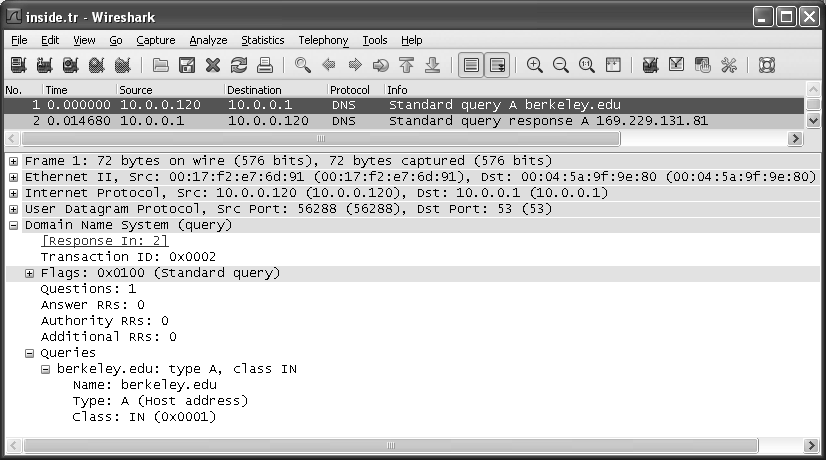
\includegraphics[width=0.7\textwidth]{imgs/11/11-10.png}
	\caption{一个 UDP/IPv4 数据报,它包含一个 DNS标准查询,即查询 berkeley.edu 相关的IPv4 地址}
\end{figure}

在跟踪记录中有两个消息:一个标准查询消息和一个标准查询响应消息。在第一条消息
(查询)中,源IPv4地址是10.0.0.120(在客户端的DHCP 分配的地址;见第6章),目的地
是10.0.0.1(DNS服务器)。查询是一个源端口为56288(临时端口)和目的端口为53(知名
DNS端口)的UDP/IPv4数据报。根据完整封装,请求是一个包含72字节的以太网帧。此
长度可以通过以下几个部分求和得到:以太网头部(14字节),IPv4头部(20字节),UDP
头部(8字节),DNS 固定头部(12字节),查询类型(2字节),查询类(2字节),加上
berkeley 和 edu 的数据标签(分别为9字节和4字节),再加上尾部的0字节。

现在讨论 DNS头部的细节,事务 ID 是0x0002,形成了DNS头部的前2个字节,位
于UDP 负载的开始处。只有一个标志(默认的递归请求)被设置,因此该消息是一个查询
消息。消息包含一个标准查询,带有一个问题。其他区段是空的。问题本身是为了查询名
称 berkeley.edu,并且正在寻找IN(互联网)类中A类型(地址记录)的信息。在收到此消
息后,运行于10.0.0.1的名称服务器进程不能直接响应,因为它不知道该地址,然后它将查
询转发至配置使用的下一个(上游)名称服务器。在本特例情况下,那个名称服务器地址为
206.13.28.12(见图11-11)。

\begin{figure}[!htb]
    \centering
	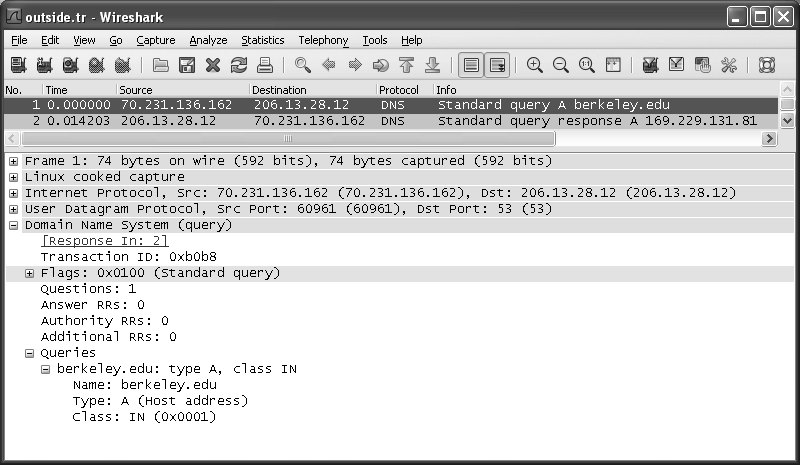
\includegraphics[width=0.7\textwidth]{imgs/11/11-11.png}
	\caption{在GW.HOME产生的DNS请求,因为递归被发送到ISP 的名称服务器}
\end{figure}

在图11-11中,我们看到了一个与客户端发出的查询相似的查询,但在这种情况下源
IPv4 地址是 70.231.136.162(ISP 端的GW.HOME 的IPv4地址)。目的地址是206.13.28.12,
是ISP提供的DNS服务器的IPv4地址,源端口是位于本地DNS服务器的临时端口
(60961)。事务ID 重新生成并设置 Oxb0b8。需要注意的是,Wireshark 指出对查询的响应
包含在数据分组2中。

图11-12中的数据分组2是我们所看到的第一个 DNS响应。首先,我们注意到,UDP
源端口号是53,但目的端口是临时端口 60961。事务ID 与查询(0xb0b8)匹配,但标志
(Flags)字段现在包含值 0x8180(响应、递归请求和可用递归全部被设置)。问题区段包含
正在提供答案的问题的一份副本,并且通常和由客户端发送的原始查询完全匹配(例如,大
小写被保留)。在回答区段有一个 RR。它是A类型(地址)的,TTL值为10分钟,数据长
度4个字节(IPv4地址的长度),其值为169.229.131.81,即我们要请求的berkeley.edu的
IPv4地址。注意,授权标志没有设置,应答的授权区段是空的。该响应基于缓存的数据,它
不是该域名的授权。此时,本地域名服务器也缓存该值(但只有10分钟,如它收到的RR中
的TTL 所说明的),并回答请求客户端(见图11-13)。

在图11-13中的响应,数据分组2很像从206.13.28.12发送的那一个,除了现在它是从
向原始客户端10.0.0.120发送的,以及事务 ID 与原始DNS 请求中的相匹配。还要
注意的是,从客户端的角度看,整个事务处理的往返时间是14.7ms 左右,而我们知道大部
分的时间(14.2ms)被本地域名服务器(GW.HOME)和ISP 的域名服务器(206.13.28.12)
之间的事务占据。

\begin{figure}[!htb]
    \centering
	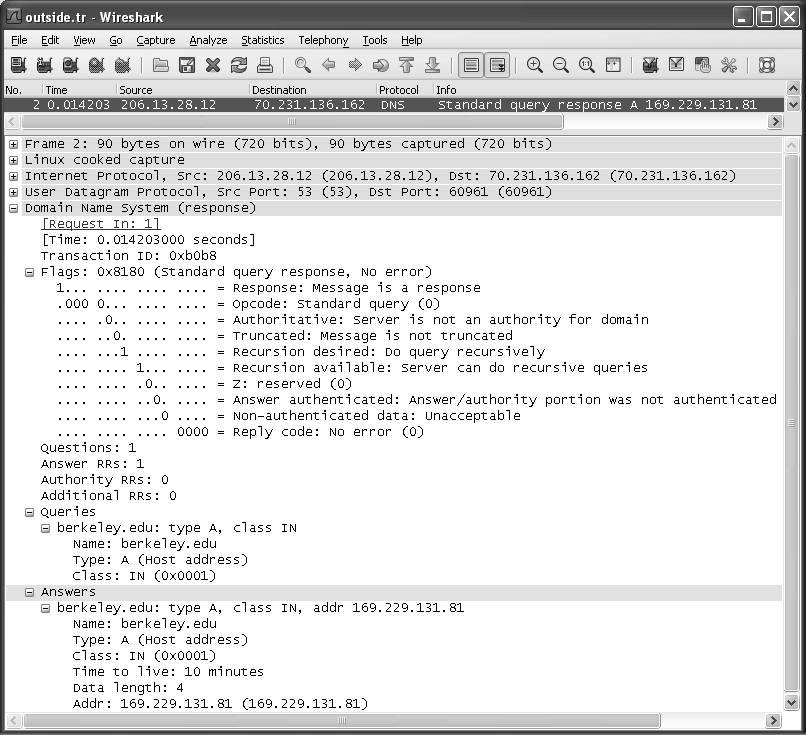
\includegraphics[width=0.7\textwidth]{imgs/11/11-12.png}
	\caption{从ISP的 DNS服务器发送到GW.HOME的一个标准的 DNS响应}
\end{figure}

\begin{figure}[!htb]
    \centering
	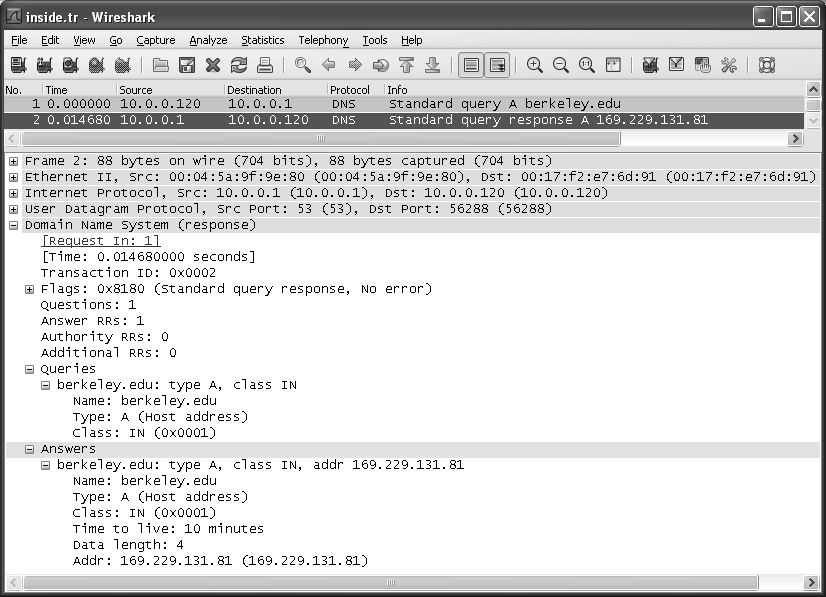
\includegraphics[width=0.7\textwidth]{imgs/11/11-13.png}
	\caption{由GW.HOME 生成去往客户端的响应。这个消息完成了递归的DNS 事务规范名称(CNAME)记录}
\end{figure}

\subsubsection{规范名称(cNAME)记录}

CNAME 记录代表规范名称(canonical name)的记录,并用于将单一域名的别名引人到
DNS 命名系统中。例如,名称 www.berkeley.edu 可能有一个CNAME记录,以映射到其他
一些机器(例如,www.w3.berkeley.edu),因此,如果 Web 服务器位于一台不同的计算机上,
世界上其他地方要找到该新系统所需要做的可能就是对DNS数据库进行一个相对简单的改
变。现在普遍的做法是使用 CNAME记录来建立公共服务的别名。因此,如www.berkeley.
edu、ftp.sun.com、mail.berkeley.edu 和www.ucsd.edu 的名称都是DNS中指向其他RR的
CNAME条目。

在一个 CNAME RR 中,RDATA 区段包含与该域名相关的“规范名称”(别名)。这样的
名称使用和其他名称相同的编码类型(例如,数据标签和压缩标签)。当一个 CNAME RR因
一个特定的名称而存在,其他数据是不被允许的\href{https://www.rfc-editor.org/rfc/rfc1912}{[RFC1912]}(除非在使用 DNSSEC;见第18
章)。CNAME RR 的域名可能不能用于规则域名能出现的所有地方(例如,作为一个 NS RR
的目标)。此外,规范名称本身可能是一个 CNAME(称为 CNAME 链),但是通常不鼓励这
么做,因为它可以导致DNS解析器使用更多的非必要的查询。然而,确实也有一些服务使
用此功能。例如,大容量站点 www.whitehouse.gov(在写作的时候)使用了Akamai公司所
提供的内容交付网络(CDN)\footnotemark。当查看这个域名时,我们找到以下内容:

\begin{verbatim}
    Linux& host -t any www.whitehouse.gov
    www.whitehouse.gov is an alias for www.whitehouse.gov.edgesuite.net.
    Linux& host -t any www.whitehouse.gov.edgesuite.net
    www.whitehouse.gov.edgesuite.net is an alias for a1128.h.akamai.net.
    Linux& host -t any a1128.h.akamai.net
    a1128.h.akamai.net has address 92.123.65.42
    a1128.h.akamai.net has address 92.123.65.51
\end{verbatim}

这样,CNAME 链就可以和DNS一起使用。然而,由于其潜在的性能影响,这样的链
通常被解析器限制在几个链接内(如5)。长链有可能是执行错误或是误解的结果,因为很难
想象在正常情况下为什么需要它们。

\begin{tcolorbox}
    有一个标准的资源记录称 DNAME(类型 39)\href{https://www.rfc-editor.org/rfc/rfc2672}{[RFC2672]}[IDDN]。 DNAME
    记录就像 CNAME 记录一样,但是是整个区域的。例如,使用一个单一的DNAME
    资源记录可以将具有 NAME.example.com 形式的所有名称映射到 NAME.newexample.
    com。然而,DNAME记录并不适用于顶层记录本身(这里的 example.com)。
\end{tcolorbox}

\subsubsection{逆向 DNS查询:PTR(指针)记录}

虽然 DNS最重要的功能是提供从名称到IP地址的映射,但是很多情况下,需要逆向
映射。例如,一个正接受传人的TCP/IP连接请求的服务器能够从传入的IP 数据报确定连接
的源IP地址,但连接本身并不携带该地址对应的名称,这样名称就必须通过其他方式查找。
幸运的是,巧妙地利用 DNS 可以提供这种能力。

PTR RR类型用于响应逆向DNS查询,当将一个 IP地址转换为其名称时,它通常是很
必要的。它以一种特殊的方式使用了特殊的 in-addr.arpa (IPv6 中为 ip6.arpa)域。考虑一个
IPv4 地址,如128.32.112.208。在分类的地址结构中(见第2章),这个地址来自于 128.32B
类地址空间。为了确定对应到这个地址的名称,首先将该地址逆转,然后添加特殊的域。本
例中,将会使用名称

 \footnotetext{内容交付网络一般包括大量同步内容缓存,它们位于网络的特定拓扑位置。CDN 可让客户访问内容提供
商的付费内容时的延迟最小。}

\begin{verbatim}
    208.112.32.128.in-addr.arpa.
\end{verbatim}

进行PTR记录的查询。实际上,这是在查询域112.32.128.in-addr.arpa. 中的“主机”208。
在本节中我们稍后将会看到更多的逆向 DNS查询的例子。

\begin{tcolorbox}
    通常使用NS、A和AAAA记录的规则DNS名称空间,不会自动与PTR记
    录支持的“逆向” 名称空间连接。因此,有一个现有的没有设置对应的逆向映射的
    前向解析(或是有一个不同的)是可能的(甚至是比较常见的)。一些服务检查两个
    方向设置的等价映射,并且在这种情况下,可能会拒绝服务。
\end{tcolorbox}

回忆一下,IPv4地址通常以“点分十进制格式”书写,IPv6地址以十六进制格式
书写(例如,169.229.131.81 和 2001:503:a83e::2:30)。这些地址可以被认为是自左到右
层次结构中存在的名称。例如,地址 169.229.131.81 有自上而下的层次结构(阅读自左
往右):169,229,131,81。通过逆转点分十进制IPv4地址,将其看作是一个DNS名
称,我们可以使用DNS来执行从IP地址到名称的映射。因此名称81.131.229.169实际
上是IPv4地址169.229.131.81的逆转。对于IPv6来说,方案是相似的,但是任何不显
示的0被展开,每个十六进制数字变成一个字符。例如,2001:503:a83e:2:30的逆转是
0.3.0.0.2.0.0.0.0.0.0.0.0.0.0.0.0.0.0.0.c.3.8.a.3.0.5.0.1.0.0.2。幸运的是,用户很少要直接输人
这些名称。

如前所述,特殊的,in-addr.arpa 域(适用于 IPv4)和.ip6.arpa(适用于IPv6)用于将支
持这些类型名称和逆向DNS 查找的PTR(“指针”)RR 连接起来。例如,考虑下面的命令:

\begin{verbatim}
    
C:\> nslookup

Default Server:

gw

Address:

\subsection{.1}
> server c.in-addr-servers.arpa

Default Server: c.in-addr-servers.arpa

Address:

196.216.169.10

> set typemptr

> 81.131.229.169.in-addr.arpa.

Server:

c.in-addr-servers.arpa

Address:

196.216.169.10

169.in-addr.arpa

169.in-addr.arpa

169.in-addr.arpa

169.in-addr.arpa

169.in-addr.arpa

169.in-addr.arpa

169.in-addr.arpa

169.in-addr.arpa

nameserver = w.arin.net

nameserver

= t.arin.net

nameserver

= dill.arin.net

nameserver

= x.arin.net

nameserver

z.arin.net

nameserver

Y.arin.net

nameserver

= u.arin.net

nameserver

= v.arin.net
\end{verbatim}

这个例子显示了如何设置.in-addr.arpa 域。根据\href{https://www.rfc-editor.org/rfc/rfc5855}{[RFC5855]},域 in-addr-servers.arpa 和
ip6-servers.arpa 分别用于形成与服务器相关的域名,并且该服务器为IPv4和IPv6提供逆向
DNS映射。截至2011年,对于每个 IP 版本有5个这样的服务器:X.in-addr-servers.arpa 和
X.ip6-servers.arpa,其中X是任意a 到f(包括)的字母。

虽然我们已经提到的10个服务器包含逆向映射的授权数据,但是它们不包含我们正在
查找的信息。在我们的例子中,第一台服务器联系了(而不是告诉我们去联系)由美国网络
地址注册管理组织(ARIN)维护的8台名称服务器之一,它可以对以 169开始的IPv4地址
授权。如果我们联系这些服务器中的一个,我们发现对于81.131.229.169.in-addr.arpa 的PTR
查询给出了以下响应:
\begin{verbatim} 
    > server w.arin.net
    Default Server: W.arin.net
    Address: 72.52.71.2
    Default Server: w.arin.net
    Address: 2001:470:1a::2
    > 81.131.229.169.in-addr.arpa.
    Server: w.arin.net
    Address: 72.52.71.2

    229.169.in-addr.arpa nameserver = adnsl.berkeley.edu.
    229.169.in-addr.arpa nameserver = phloem.uoregon.edu.
    229.169.in-addr.arpa nameserver = aodnsl.berkeley.edu.
    229.169.in-addr.arpa nameserver = adns2.berkeley.edu.
\end{verbatim}

这里我们可以推测,拥有网络前缀169.229/16的教育机构是伯克利大学,该大学维护了三个
域名服务器,覆盖了它的 in-addrarpa 空间,并且俄勒冈大学还提供一个副本。通过继续联系
这些服务器中的一个,我们找到了答案(这次使用 Linux版本的 nslookup,输出略有不同):

\begin{verbatim}
    Linuxe nslookup
    > set type=ptr
    > server adnsl.berkeley .edu
    Default Server: adnsl.berkeley.edu
    Address:128.32.136.3#53
    Default Server:adnsl.berkeley.edu
    Address:2607:f140:ffff:fffe::3#53
    > 81.131.229.169.in-addr.arpa.
    Server:adnsl.berkeley.edu
    Address: 128.32.136.3#53
    81.131.229.169.in-addr.arpa name = webfarm.Berkeley.EDU
\end{verbatim}

这里我们得到所期待的结果,即 IPv4地址169.229.131.81 的名称为 webfarm.Berkeley.
EDU。DNS 服务器使用端口53,如IP 地址后的\#53所示。使用UDP/IPv4(相对于 UDP/
IPv6)访问 DNS仍然可以通过使用“四A”(AAAA)DNS 记录提供IPv6地址的映射,因为
我们可以看到服务器的IPv6地址是 2607:f140:ffff:fffe::3,从输出来看这是很显然的。

如果没有 DNS树的单独分支来处理地址到名称的翻译,基本上就没有办法完成逆向翻
译,除非从树根开始尝试每个顶级域名。鉴于互联网的当前规模,这显然是不合理的选择。
in-addr.arpa 解决方案是有效的,并且还非常高效,虽然IPv4/IPv6地址的逆转字节和特殊域
的域名令人困惑。幸运的是,如前所述,用户通常可以避免输人或使用它们。即使是应用程
序作者,通常也不必操作地址来执行逆向查询,因为库函数(如C库函数getnameinfo())执
行这项工作。

值得一提的是,PTR 查询已经成为全球 DNS服务器的一个重要问题。考虑一个家庭网
络,它使用一类私有地址前缀,如10.0.0.0/8(IPv4)或fc00:/7(IPv6)。当一个系统接收到
相同私有编址子网的另一个系统传入的连接请求时,它可能希望将源地址解析名称,并且
通过执行PTR查询来完成。如果查询没有得到本地DNS服务器的回答,那么它可能会传播
到全球互联网。出于这个原因(以及一些其他原因),\href{https://www.rfc-editor.org/rfc/rfc6303}{[RFC6303]} 指定本地名称服务器—
尤其是那些连接到互联网且使用私有IP地址的网络中运行的服务器,为在\href{https://www.rfc-editor.org/rfc/rfc1918}{[RFC1918]}和
「RFC41931中为IPv4 和 IPv6 定义的私有地址空间提供PTR 映射(即分别为 IN-ADDR.ARPA
和 D.F.IP6.ARPA)。

\subsubsection{无类别 in-addr.arpa 委托}

当组织加入互联网,并获得授权来填充部分 DNS名称空间时,它们往往也获得与它们
互联网上的IPv4地址相对应的部分 in-addr.arpa 名称空间的授权。在UC伯克利分校例子中,
授权包括网络前缀169.229/16,使用旧日的术语,即为“B类”网络号169.229。因此,UC伯
克利分校预计会使用名称以 229.169.in-addr.arpa结尾的PTR记录来填充部分DNS树。分配
给该组织的地址前缀是以前的A、B或C类样式时,这会工作得很好,这些旧的分类中位数
是8的整数倍。然而,现在许多组织有大于24位或大于16(但少于24)位的前缀长度。在
这些情况下,地址范围就不易写为IP地址的简单逆转形式。相反,一些传输网络前缀长度
的方法也必须包括在内。

\href{https://www.rfc-editor.org/rfc/rfc2317}{[RFC2317]}给出了实现的标准方法,即添加前缀长度到逆转后的字节组中,并使用它作
为域名中的第一个标签。例如,假设一个站点分配的前缀为12.17.136.128/25,即包含128
个地址的前缀。根据\href{https://www.rfc-editor.org/rfc/rfc2317}{[RFC2317]},应提供两种类型的记录。首先,按照下列方式,为形式为
X.136.17.12.in-addr.arpa(其中X至少为128且不超过255)的每一个名称创建一个 CNAME
RR,可能由站点的ISP 维护:

\begin{verbatim}
    128.136.17.12.in-addr.arpa. canonical name =
                                128.128/25.136.17.12.in-addr.arpa.

    129.136.17.12.in-addr.arpa. canonical name =
                                129.128/25.136.17.12.in-addr.arpa.
    ...
    255.136.17.12.in-addr.arpa. canonical name =
                                255.128/25.136.17.12.in-addr.arpa.
\end{verbatim}

这里我们可以看到网络前缀是如何使用域名中第二个标签相关的“/” 符号编码的(在
这个例子中)。这些条目通常放在ISP 处,允许对于非字节对齐地址范围的委托。在这个例
子中,客户现在能够为区域128.128/25.136.17.12.in-addr.arpa 提供映射了。我们可以按以下
方式跟踪委托:

\begin{verbatim}
    
C:\> nslookup

Default Server:

gW

Address: 10.0.0.1

> server f.in-addr-servers.arpa

Default Server: f.in-addr-servers.arpa

Addresses: 193.0.9.1

> set type=ptr

> 129.128/25.136.17.12.in-addr.arpa.

Server:

f.in-addr-servers.arpa

Address: 193.0.9.1

12.in-addr.arpa nameserver = dbru.br.ns.els-gms.att.net

12.in-addr.arpa nameserver = cbru.br.ns.els-gms.att.net

12.in-addr.arpa nameserver = cmtu.mt.ns.els-gms.att.net

12.in-addr.arpa nameserver = dmtu.mt.ns.els-gms.att.net

> server dbru.br.ns.els-gms.att.net.

Default Server:

dbru.br.ns.els-gms.att.net

Address: 199.191.128.106

> 129.128/25.136.17.12.in-addr.arpa.

128/25.136.17.12.in-addr.arpa

128/25.136.17.12.in-addr.arpa

nameserver = ns2.intel-research.net

nameserver= ns1.intel-research.net

>

SerVer

n81.intel-research.net.

Server:

nsl.intel-research.net

Address: 12.155.161.131

> 129.128/25.136.17.12.in-addr.arpa.

129.128/25.136.17.12.in-addr.arpa

name

= dmz.slouter.seattle.intel-research.net

128/25.136.17.12.in-addr.arpa

nameserver = bldmzsvr.berkeley.intel-research.net

128/25.136.17.12.in-addr.arpa

nameserver

= Sldmzsvr.intel-research.net

bldmzsvr.berkeley.intel-research.net internet address = 12.155.161.131

sldmzsvr.intel-research.net internet address = 12.17.136.131
\end{verbatim}

在这个例子中,我们希望找出与IPv4地址12.17.136.129相关的主机名称。我们已
经看到,它有一个 CNAME RR 指向规范名称129.128/25.136.17.12.in-addr.arpa.。 我们
指示解析器使用一台根服务器(F),并设置查询类型为 PTR RR。至此,我们请求解析
129.128/25.136.17.12.inaddr.arpa.。根名称服务器没有该信息,它不执行递归,所以它返回域
12.in-addr:arpa.的授权服务器的名称。选择它们之一(DBRU),再次尝试解析我们的问题。
这一次我们发现两个域名服务器(nsl 和ns2)。选择其中之一,我们能够解析该PTR 请求。
解析出的名称內 dmz.slouter.seattle.intel-research.net。

\subsubsection{权威 (SOA)记录}

在DNS中,每个区域有一个授权记录,使用称授权启动(SOA)的RR类型。这些
记录提供部分 DNS名称空间和服务器之间的授权联系,该服务器允许对地址和其他信息进
行查询以提供区域信息。SOA RR 用于识别主机的名称,提供官方永久性数据库、负责方的
e-mail 地址(“.”用来代替@)、区域更新参数和默认 TTL。默认 TTL 应用到区域中的 RR,
不用为每个 RR 指定TTL 值。

区域更新参数包括一个序列号、更新时间、重试时间和终止时间。每当要改变区域内容
时,序列号通常由网络管理员增加(至少1)。辅助服务器使用它来确定是否应该启动区域传
输(当它们没有序列号最大的区域内容的副本时)。更新时间告诉辅助服务器,在从主服务器
检查SOA记录之前需要等待的时间以及它的版本号,以确定是否需要区域传输。重试时间
和终止时间是在区域传输失败的情况下使用的。重试时间值给出辅助服务器重试前需要等待
的时间(秒)。终止时间是辅助服务器在放弃之前保持重试区域传输的上限(秒)。如果它放
弃了,这样的服务器停止响应对该区域的查询。一般情况下,一个区域可以包含混合的IPv4
和IPv6数据,并可以使用任意版本的IP来访问。在这个例子中,我们使用IPv6(使用只有
IPv6 的 Windows 主机上的 nslookup):

\begin{verbatim}
    
C:\> n8lookup

Default Server:

gw

Address:

fe80::204:5aff:fe9f:9e80

> set type=8oa

> berkeley.edu.

Server:

gW

Address:

fe80::204:5aff:fe9f:9e80

Non-authoritative answer:

berkeley.edu

primary name server = ns-masterl.berkeley.edu

responsible

mail

addr

hostmaster.berkelev.edu
serial = 2009050116

refresh = 10800 (3 hours)

retry

= 1800 (30 mins)

expire = 3600000 (41 days 16 hours)

default TTL = 300 (5 mins)

> server adnsl.berkeley .edu.

Default Server:

adnsl.berkeley.edu

Addresses: 2607:f140:ffff:fffe::3

128.32.136.3

> berkeler.edu.

Server:

adns1.berkeley.edu

Addresses: 2607:£140:ffff:fffe::3

128.32.136.3

berkeleyedu

Primary name server = ns-masterl.berkeley .edu

responsible mail addr = hostmaster.berkeley.edu

serial

= 2009050116

refresh = 10800 (3 hours)

retry

= 1800 (30 mins)

expire = 3600000 (41 days 16 hours)

default TTL = 300 (5 mins)

berkeley.edu

nameserver = ns.v6.berkeley.edu

berkeley.edu

nameserver = aodnsl.berkeley.edu

berkeley.edu

nameserver = adns2.berkeley.edu

berkeley.edu

nameserver = phloem.uoregon.edu

berkeley.edu

nameserver = adnsl.berkeley.edu

berkeley.edu

nameserver = ucb-ns .NYU.edu

ns.v6.berkeley.edu

internet address = 128.32.136.6

ns.v6.berkeley.edu

AAAA IPv6 address = 2607:f140:ffff:fffe::6

adnsl.berkeley.edu

internet address = 128.32.136.3

adnsl.berkeley.edu

AAAA IPV6 address = 2607:f140:ffff:fffe::3

adns2.berkeley.edu

internet address = 128.32.136.14

adns2.berkeley.edu

AAAA IPV6 address = 2607:f140:ffff:fffe::e

aodnsl.berkeley.edu

internet address = 192.35.225.133

aodns1.berkeley.edu

AAAA IPV6 address =

2607:f010:3E8:8000:214:4fff:fe45:e6a2

phloem.uoregon.edu

phloem.uoregon.edu

internet address = 128.223.32.35

AAAAA

IPv6 address = 2001:468:d01:20::80df:2023

\end{verbatim}
这里我们可以看到,我们不仅收到SOA记录,而且也收到了6个授权域名服务器的列
表,以及其中5个(NYU服务器的地址没有给出,因为NYU.edu 的胶记录可能在由不同服
务器支持的不同的区域里)的IPv4/IPv6地址(胶记录)。由于这是我们已经看到的更多有趣
的响应中的一个,让我们看一下与发送到授权名称服务器 adnsl.berkeley.edu 的请求相对应
的分组内容(见图11-14)。

此记录包含两个分组,我们已选择显示答复,它是两个中更引人关注的。一个 SOA RR
查询从本地系统的全球范畴的IPv6地址2001:5c0:1101:ed00:5571:5f81:e0a6:4978 发送到主
机 2607:f140:fff:fffe::3 (adns1.Berkeley.EDU)。响应在一个总长度为491字节(负载长度字
段是451)的IPv6数据报中运载。该特分组包含IPv6头部(40字节)、UDP头部(8字节)
以及 DNS消息(443字节)。DNS消息包含1个问题、1个答案、6个授权RR 和10个附加
的 RR。

问题区段包含标签 berkeley 和edu,18个字节长。回答区段包含前面描述过的 berkeley.
edu 域名的相关信息,并且由于问题区段的内容,它能够利用压缩标签。该区段的总长度是
58字节。授权区段包含6个识别名称服务器的 NS记录。该信息另需135字节。额外信息区
段包括5个A记录和5个 AAAA 记录,共220个字节。每个 AAAA记录的RDATA 字段的
长度为16字节,因此,尽管IPv6地址可以以带有“:”的文本形式来节省空间,但是它在
分组中并非如此编码。相反,使用了全部的128位地址。

\begin{figure}[!htb]
    \centering
	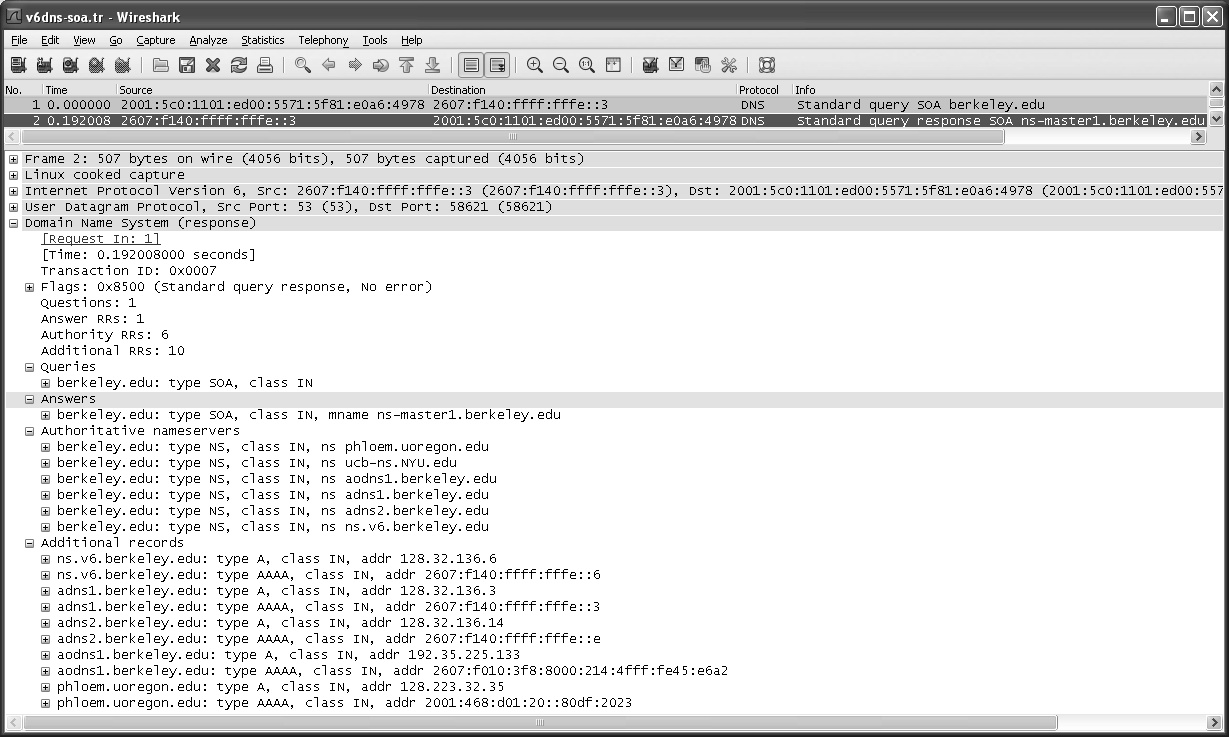
\includegraphics[width=0.7\textwidth]{imgs/11/11-14.png}
	\caption{使用IPv6对一个SOA 记录 DNS 查询的响应。响应包括该区域的 IPv4 和 IPv6地址}
\end{figure}

\subsubsection{邮件交换(MX)记录}

MX记录提供了邮件交换器(mail exchanger)的名称,邮件交换器为在简单邮件传输协
议(SMTP)\href{https://www.rfc-editor.org/rfc/rfc5321}{[RFC5321]}中愿意代表与域名相关的用户接收传入电子邮件的主机。当互联网仍
在发展时,一些站点没有固定连接,而是拨号连接到具有固定互联网连接的主机。在这样的
情况下,当电子邮件在传输过程中目的地可能从网络上断开,因此另一台主机必须保留该邮
件,直到目的地连接上为止。这是在 DNS 中包含MX记录的一个原因,即使真实目的地不
可用,也允许发送方主机将电子邮件交付给中介(“中继服务器”)。现在MX记录仍然在使
用,邮件代理更愿意将电子邮件交付给 MC记录中列出的与特定域名相关的主机。
MX记录包括优先级(preference) 值,因此对于一个特定的域名,多个MX记录可以
同时出现。优先级值允许发送代理按优先顺序(较小的是更可取的)排序主机,以决定哪个
主机用作电子邮件的目的地。例如,我们可以再次使用 host 命令查询 DNS 中与域名cs.ucla.
edu 相关的 MX 记录:

\begin{verbatim}
    Linux% host -t MX cs.ucla.edu ns3.dns.ucla.edu
    Using domain server:
    Name: ns3.dns.ucla.edu
    Address: 2607:f600:8001:1::ff:fe01:35#53
    Aliases:

    cs.ucla.edu mail is handled by 13 Pelican.cs.ucla.edu.
    cs.ucla.edu mail is handled by 3 Moa.cs.ucla.edu.
    cs.ucla.edu mail is handled by 13 Mailman.cs.ucla.edu.
\end{verbatim}

在这里我们可以看到,邮寄到person@cs.ucla.edu 的电子邮件由在 DNS中配置的三台
邮件服务器之一处理。所有的这些邮件服务器是cs.ucla.edu 域的一部分,但一般情况下,邮
件服务器不必与它们正在处理的电子邮件有相同的域。这三个服务器可分为两部分:一部分
优先级为3,一部分优先级为13。优先级编号较小的服务器是首选的,所以发送方首先尝试
Moa.cs.ucla.edu。如果失败,它会随即选择 Pelican或 Mailman 进行尝试。

很可能MX记录的目标主机都不可达。这是一种错误状态。也可能现在没有MX记录,
但有该域名的CNAME、A或AAAA 记录。如果有一个 CNAME记录,CNAME 的目标是用
来代替原来的域名。如果有 A或AAAA记录,邮件代理可以连接到这些地址。每个被认为
其优先级为0(称为隐式 (implicit)MX)。MX记录目标必须是解析 A 或AAAA 记录的域名;
它们不能指向 CNAME\href{https://www.rfc-editor.org/rfc/rfc5321}{[RFC5321]}。

\subsubsection{打击垃圾邮件:发送方策略框架(SPF)和文本(TXT)记录}

对于发出的电子邮件,MX记录允许 DNS帮助确定邮件中继和域名服务器的名称。最
近,DNS已被接收邮件代理利用,以确定哪些中继或发送邮件服务器被授权以发送来自特定
域名的邮件。这被用来帮助打击垃圾邮件(不需要的电子邮件),这些垃圾邮件由假装成经授
权的邮件发送方的流氓邮件代理发送。

邮件服务器收到的电子邮件被拒绝、存储或转发到另一个邮件服务器。拒绝发生的原因
有很多,如协议错误或接收方缺乏可用存储空间。因为发送方邮件客户端不是发送电子邮件
的合适方也可以被拒绝。这种能力由发送方策略框架(Sender Policy Framework, SPF)支持,
并记录在\href{https://www.rfc-editor.org/rfc/rfc4408}{[RFC4408]}中,这是一个实验性的 RFC。还有另外一个称发送方 ID (Sender ID)
\href{https://www.rfc-editor.org/rfc/rfc4406}{[RFC4406]}的框架,它结合了 SPF的功能。它也是实验性的,但是没有广泛部署。

SPF 的第一个版本使用 DNSTXT或SPF(类型99)资源记录。由域拥有者建立记录,
并在DNS中发布,以指明哪些服务器被授权发送来自该域的邮件。虽然在某种意义上SPF
记录类型是一个更“合适”携带 SPF 相关信息的地方,但是一些 DNS客户端的实现没有适
当地处理SPF记录,所以为了避免这一情况,使用TXT记录。TXT记录保存与域名相关的
简单的字符串。从历史上看,它们保留人类理解的字符串,以帮助调试或确定拥有者或域的
位置。现在,它们通常由程序处理,如SPF 应用程序。

SPF 支持丰富的语法来表达一些准则,这些准则用于匹配传入的邮件信息和承载它的
连接的详细情况。例如,UC伯克利分校使用以下的SPF项(为清晰起见,有些行已经隐藏
起来):

\begin{verbatim}
    Linux% host -t txt berkeley.edu
    berkeley.edu descriptive text
            "v=spf1 ip4:169.229.218.128/25 ip6:2607:F140:0:1000::/64
            include:outboundmail.convio.net ~all"
\end{verbatim}

在这个例子中,所提供的信息是对SPF版本1的(通过版本字段中v=spf1 字符串来说
明),并且使用TXT RR。当接收邮件代理接收到据称来自于域berkeley.edu 的电子邮件时,
它对berkeley.edu 域执行TXT类型记录的DNS查询。文本记录的值包含匹配的准则(称
机制(mechanism))和其他信息(称为修饰符(modifiers))。在每个机制之前是一个限定符
(qualifier),用以确定匹配机制的结果。处理SPF记录使用称为 check\_bost()的函数。该函
数对各种机制进行评估,当遇到第一个匹配的机制时完成。最终,check\_hostO提供以下返
回值之一:None、Neutral、Pass、Fail、SoftFail、TempBrror 和 PermError。None 和 Neutral
返回值说明没有信息可用,或是有信息可用但是没有声称的结果。这些按完全相同的方式
处理。Pass 说明一个匹配将如下一段描述的。Fail说明发送方主机没有被授权从该域发送邮
件。SoftFail有点模糊,但根据\href{https://www.rfc-editor.org/rfc/rfc4408}{[RFC4408]},它被视为“介于‘Fail’和‘Neutral’之间”。
TempError 返回值表示某些可能减弱的暂时性失败(如通信故障)。PermError 返回值表示
SPF 的配置中存在问题,通常是因为有缺陷的域 TXT或SPF记录。

在例子中,自从左向右阅读,字符串v=spfl 是一个修饰符,说明 SPF的版本是1。ip4
机制说明SMTP发送方拥有一个前缀169.229.218.128/25的IPv4地址。ip6机制说明
发送方主机的IPv6地址前缀2607:F140:0:1000:/64。最后,include 机制通过引用包含
outboundmail.convio.net TXT 记录:

\begin{verbatim}
    Linux% host -t txt outboundmai1.convio.net
    outboundmail.convio.net descriptive text
            “v=spf1 +ip4:66.45.103.0/25 +ip4:69.48.252.128/25
            +ip4:209.163.168.192/26 ~all"
    outboundmail.convio.net descriptive text
            "spf2.0/pra
            +ip4:66.45.103.0/25 +ip4:69.48.252.128/25
            +ip4:209.163.168.192/26 ~all"
\end{verbatim}

\begin{tcolorbox}
    这些TXT记录均适用于 SPF 和发送方ID(在版本区段使用值spf2.0/pra)。第一
    条记录由 SPF使用。“+”限定符表明匹配结果为Pass。任何无限定符的机制假定拥有“+”
    限定符。其他可能的限定符包括- (Fail)、~ (Soft Fail)和?(Neutral)。如果没有匹配机制
    产生Pass结果,最终机制(all)匹配任何条件。all准则之前的波浪符号(~)说明如果 all
    是唯一匹配的机制,那么应该生成SoftFail返回值。软故障的具体处理方式依赖于接收电子
    邮件的软件。请注意,即使有 SPF 的支持,验证也只由发送方域和系统提供,而不是发送用
    户。在第18 章我们将着眼于 DKIM,它提供类似 SPF的功能,但使用加密进行身份验证。
\end{tcolorbox}

\subsubsection{选项(OPT)伪记录}

如前所述,连同 EDNSO也定义了特的 OPT伪RR\href{https://www.rfc-editor.org/rfc/rfc2671}{[RFC2671]}。就某种意义而言,它
是“假的”,它仅适用于单一DNS消息的内容,而且不是常见的DNS RR数据。因此,OPT
RR 不被缓存、转发或持续存储,它们可能在 DNS消息中只出现一次(或不出现)。如果出
现在 DNS消息中,可以在额外消息区段中发现它。

一个OPT RR 包含10个字节的固定部分,随后是一个可变部分。固定部分包括表示
RR类型(41)的16位,表示 UDP 负载大小的16位,构成一个扩展的RCODE 字段和 Flag
域的32位,以及指出以字节为单位的可变部分大小的16位。这些字段与传统的RR 中的
Name、Type、Class、TTL 和 RDLEN 有相同的相对位置关系(见图11-8)。OPT RR 在名字
字段使用空域名(0个字节)。扩展RCODE 和Flags域(32位,对应于图11-8中的TTL字
段)被再分成两个8位域,一个用于保留额外的8个高位,扩充图11-3中的RCODE字段,
一个为版本字段(当前设置0表示EDNSO)。剩余的16位尚未定义,必须为0。额外的8
位提供了一个可能的DNS错误类型的扩展集,这些值在表11-4中给出。(注意值16由两个
不同的RFC定义。)

\begin{verbatim}
    值
    
    16
    
    16
    
    17
    
    18
    
    19
    
    20
    
    21
    
    名称
    
    BADVERS
    
    BADVERS
    
    BADKEY
    
    BADTIME
    
    BADMODE
    
    BADMODE
    
    BADALG
    
    表11-4 扩展 RCODE 值。大部分被用来支持安全扩展
    
    参考
    
    描述和目的
    
    \href{https://www.rfc-editor.org/rfc/rfc2671}{[RFC2671]}
    
    \href{https://www.rfc-editor.org/rfc/rfc2845}{[RFC2845]}
    
    \href{https://www.rfc-editor.org/rfc/rfc2845}{[RFC2845]}
    
    \href{https://www.rfc-editor.org/rfc/rfc2845}{[RFC2845]}
    
    \href{https://www.rfc-editor.org/rfc/rfc2930}{[RFC2930]}
    
    \href{https://www.rfc-editor.org/rfc/rfc2930}{[RFC2930]}
    
    IRFC2930]
    
    坏 EDSN版本
    
    坏TSIG 签名(见第18章)
    
    坏TSIG 密钥(见第18章)
    
    坏TSIG 签名(时间问题;见第18章)
    
    坏TKEY 模式(见第18章)
    
    重复密钥名称(见第18章)
    
    不支持的算法(见第18章)
\end{verbatim}

正如我们已经提到的,OPT RR 包含可变长度的RDATA 字段。该字段用来存放属性-
值对的扩展列表。当前属性、意义和定义的RFC的集合都由IANA[DNSPARAMS]维护。一
个称为 NSID(EDNS选项代码3)\href{https://www.rfc-editor.org/rfc/rfc5001}{[RFC5001]}的选项,表示一个响应 DNS服务器的特殊标
识值。该值的格式没有标准定义,但是DNS 服务器的系统管理员可以配置。任播地址用于
确定一组服务器时,这种功能可能是很有用的。NSID 能够使用非发送方的IP地址的一个值
识别出一台特定的响应服务器。当我们在第18章查看 DNSSEC时,将看到更多 OPT RR 和
EDNSO用法的例子。

\subsubsection{服务记录}

\href{https://www.rfc-editor.org/rfc/rfc2782}{[RFC2782]}定义了服务(SRV)资源记录。SRV RR 推广了MX记录的格式,以描述主机、
协议和用于连接特定服务的端口号。SRV RR 的一般结构如下:

\begin{verbatim}
    \_Service. Proto.Name TTL IN    SRV Prio    Weight  Port    Target
\end{verbatim}

Service 标识符是一个服务的正式名称。Proto 标识符是用于访问服务的传输协议,通常
是TCP或UDP。TTL值是一个传统 RR的 TTL,IN和SRV 分别表明互联网类和 SRV RR类
型。Prio值是一个16位的无符号值,与MX记录中的优先权值作用差不多(越小的的数字
表示越高的优先级)。Weight 值用于在优先级相等的几个 RR 中做出选择。基本思路是,权
值用作加权概率来为负载平衡选择特定的条目,因此较大的权值表明更大的选择概率。Port
是TCP或UDP(或其他传输协议的)端口号。Target 是提供服务的目标主机的域名。Name
标识符是一个包含域,其中可以找到一个特定的服务。SRV 记录的目的之一是确定何时在一
个域中的多个单独的服务器上支持相同的服务。

例如,如果一个客户想要使用TCP 协议确定域example.com 中 ladap 服务可用的主机
和端口,它会使用域名\_Idap.\_tcp.example.com执行SRV记录的查询。这里是一个真实的
例子:

\begin{verbatim}
    Linux% host -t srv \_1dap.\_tcp.openldap.org
    \_ldaptcp.openldaporg has SRV record 0 0 389 www.openldap.org
\end{verbatim}

在这个例子中,我们通过TCP,在域openldap.org 中查找提供轻量级目录访问协议
(LDAP)服务的服务器。我们发现,可以使用TCP端口389(默认的LDAP端口),在服务器
www.openldap.org 上访问。Priority 和 Weight 值为0,因没有替代的服务器。

\href{https://www.rfc-editor.org/rfc/rfc2782}{[RFC2782]}没有 SRV Service 和 Proto值指定一个新的IANA 注册。所以,默认情况
下,名称与IANA 的“服务名称和传输协议端口”[ISPR]注册中保存的名称相对应,Proto 值
为\_tcp 或\_udp,但也有少数例外。[RFCS509]使用以下的 SRV Service 和 Proto 名称为基于
SIP 的在场和即时通信建立约定:\_im.\_sip 和\_pres\_sip。\href{https://www.rfc-editor.org/rfc/rfc6186}{[RFC6186]}为电子邮件用户代理定
义了下面的 SRV Service 名称,以便容易地发现IMAPS、SMTP、IMAP 和 POP3服务器的联
系信息(当设置电子邮件客户端时,通常前两个是优先考虑的):\_submission,\_imap,\_imaps,
\_Pop3,\_Pop3s。虽然\href{https://www.rfc-editor.org/rfc/rfc6186}{[RFC6186]}没有要求这些名称使用TCP 作为相应的Proto 值,但是这
是目前唯一的真正选项。例如,用户配置一个新的邮件用户代理(MUA,本质上是一个电
子邮件程序),可能只指定域名 example.com。然后MUA实现可能至少为\_submission.\_t
example.com 和\_imaps\_tcp.example.com 执行 DNS查询。

\subsubsection{名称授权指针记录}

当DNS支持动态委托发现系统(DDDS)\href{https://www.rfc-editor.org/rfc/rfc3401}{[RFC3401]}时,使用名称授权指针(NAPTR)
RR类型。一个 DDDS一般是抽象的算法,它将动态检索字符串转换规则应用于应用程序提
供的字符串,并经常使用结果定位资源。每个 DDDS 应用为其特定的使用情况定制一般的
DDDS规则的操作。一个DDDS 包括一个规则数据库和一组用于形成字符串的算法,该字
符串和数据库一起产生输出字符串。DNS就是这样一个数据库\href{https://www.rfc-editor.org/rfc/rfc3403}{[RFC3403]},在其中 NAPTR
资源记录类型用来保存转换规则。一个这样的DDDS 应用程序已经被定义用来和DNS一起
处理跨国电话号码,并使用 ENUM(见11.5.6.12节)将它们转换为标准的统一资源标识符
(URI)格式\href{https://www.rfc-editor.org/rfc/rfc3986}{[RFC3986]}。

在一个 DDDS 中,算法\href{https://www.rfc-editor.org/rfc/rfc3402}{[RFC3402]}指如何通过数据库中包含的规则处理应用唯一字
符串(AUS)。结果可以是一个终结字符串(terminal string)(完整的输出)或另一个(非终结)
字符串,它用于检索应用到AUS的另一个规则。总之,该集合形成了一个强大的字符串!
写系统,可用于编码有足够正则语法的几乎任意串。该算法的本质如图11-15所示。

图11-15所示的过程,开始时将“第一条众所周知的规则”(frst Well-Known Rule)应用
于AUS,AUS 对于每个应用是唯一的。结果形成一个关键字,用于从数据库中
检索另一个规则。规则是字符串重写模式和标志,该标志应用于 AUS,但是
从来不应用于重写字符串的结果。它工作的特定方式依赖于应用程序,但规则
通常是正则表达式的替换,类似于使用UNIX sed 程序[DR97]。当使用 DNS作
为支持DDDS的数据库时\href{https://www.rfc-editor.org/rfc/rfc3403}{[RFC3403]},
这正是我们感兴趣的情况,关键字是域名,规则存储于NAPTR资源记录中。
每个 NAPTR RR 包含以下字段:顺序、优先级、标志、服务、正则表达式(有
时简写为 Regexp)、替换。

DDDS算法的抽象操作。允许非终结记录形成循环。每次迭代都涉及应用唯一字符串的
重写操作

顺序字段是16位无符号整数,指定哪一个NAPTR 记录在其他之前使用
(较小的数字比较大的那些更优先),因DNS架构不保证任意特定资源记录
集的排序。优先级字段用来影响含有相同顺序号的记录的顺序。顺序字段表
明在 RR上施加强制性的顺序,而优先级是建议性的。标志字段包含来自集合
A~Z和0~9的单个字符的无序列表(大小写不敏感的)。使用NAPTR 记录
的特定的应用程序(例如 ENUM,将在
下一节描述),定义标志字段的解释。服务字段由应用程序定义,用以说明哪种类型的服务
正在被描述。正则表达式字段包含一个替换表达式,该表达式应用于AUS 以形成另一个服
务器的标识,用于另一个 NAPTR 查找(非终结情况)或输出字符串(终结情况)。替换字段
(只有当正则表达式不存在时才存在)表示要查询 NAPTR记录的下一个服务器。它被编码为
一个独立的FQDN(在DNS消息中没有使用名称压缩)。因历史的原因,在NAPTR RR的发
展过程中,这两个最后(互斥)字段的用途非常相似。

为了更好地理解 NAPTR处理如何与应用程序一起工作,我们将会简单地看一下 ENUM
和SIP DDDS 应用程序、URI/URN DDDS 应用程序,以及称 S-NAPTR 和 U-NAPTR的常
规NAPTR的替代选择。指定一个 DDDS 必须指定应用程序的AUS、第一条众所周知的规
则、期望输出、有效的数据库、标志和服务参数。

\subsubsection{ENUM 和 SIP}

在 ENUM DDDS[R06]\href{https://www.rfc-editor.org/rfc/rfc6116}{[RFC6116]} \href{https://www.rfc-editor.org/rfc/rfc6117}{[RFC6117]}\href{https://www.rfc-editor.org/rfc/rfc5483}{[RFC5483]}中,将电话号码映射到URI
信息,AUS 是一个E.164格式的电话号码(最多15个数字,以“+”字符开始)。初始的
“+”字符将ENUM DDS 中使用的E.164号码和来自其他名称空间的号码区别开来。第一
个众所周知的规则,首先移除AUS 中的任意破折号或其他非数字字符。DDDS的数据库是
DNS,关键字是从 AUS中按如下方式创建的域名:点(.)字符插入到每个数字之间,将结
果逆转。然后添加后缀.e164.arpa。例如,E.164号码+1-415-555-1212 将会被转换为密钥
2.1.2.1.5.5.5.5.1.4.1.e164.arpa。生成的域名用于查询 NAPTR记录。

最终的输出可能经过图11-15所示 DDDS算法的多个循环,是一个绝对的URI(非相
对)。定义的唯一标志是U标志,表明产生一个 URI 的终结规则。没有任何标志说明是非终
结的规则,有时也称非终结 NAPTR (Non-Terminal NAPTR,NTN)。服务参数在 NAPTR
记录的 Service 字段中编码,其形式力 E2U+Service,即来自字符串 E2U(E.164 中指向 URI
的指示器)加上提供与该号码相关的特定服务的信息的 Service 名称子域。它们一起形成了
enumservice(枚举服务)标识符,这样的服务向 IANA [ENUM]\href{https://www.rfc-editor.org/rfc/rfc6117}{[RFC6117]}注册并且已经创
建了许多,包含传真、即时通信和存在指示器的枚举服务。

为了看到这一切是如何工作的,我们可以构造一个对于号码+420738511111 的查询,
号码位于捷克的俄斯特拉法大学(为清晰起见,很多行隐藏了):

\begin{verbatim}
    Linux% host -t naptr 1.1.1.1.1.5.8.3.7.0.2.4.e164.arpa
    1.1.1.1.1.5.8.3.7.0.2.4.e164.arpa has NAPTR record
            50 50 "u""E2U+sip" "!^\\+(.*)$!sip:\\1@osu.cz!"
    1.1.1.1.1.5.8.3.7.0.2.4.e164.arpa has NAPTR record
            100 50 "E2U+sip""!^\l+(.*)$!sip:\\1@cesnet.cz!"
    1.1.1.1.1.5.8.3.7.0.2.4.e164.arpa has NAPTR record
            200 50 "u""E2U+h323" “!^\\+(.*)$!h323:\\1@gklext.cesnet.cz!"
\end{verbatim}

这里我们看到在 ENUM DDDS 应用中三个 NAPTR 记录的内容,两个用于SIP服务,一个
用于 H.323服务,它们用于互联网电话。SIP 条目的序列号50和100,H.323条目的序列
号为200,同时显示了如何使用 ENUM 和 NAPTR记录来拥有多个与单一电话号码相关的服
务,以及 NAPTR记录的提供者如何指出提供相同服务的多个网关的优先级顺序。

\begin{tcolorbox}
    SIP 是IETF 指定的用于信令的协议,因使得多媒体客户端和服务器的连接便
    利而特别流行。H.323是ITU 指定的协议,用于多媒体会议和通信,包括一个信令
    子协议。它广泛实现于电话会议设备中。本例以及随后的例子中,host程序产生的
    输出可以用作如BIND 的DNS服务器的区域文件的输入。因此,输出显示额外的转
    义“\\”宇符(显示为“\\”),它们在实际的服务器提供的DNS 响应中并不存在。
\end{tcolorbox}

为了更好地了解NAPTR记录规则如何应用到AUS,我们将着眼于前面例子中的第
二个SIP 记录。执行DNS查询和收到NAPTR RR后,出现在第一个和第二个“!”宇符
之间的字符串用作一个正则表达式匹配和替换。这样,字符串+420738511111与正则表
达式\verb|八\+(*)$|相匹配。根据正则表达式匹配的规则,匹配成功,所以字符串重写规则变为
sip: 1@cesnet.cz。特殊变量\\1被与圆括号()之间包含的第一个正则表达式相匹配的子串
替换,在这种情况下,即为AUS中除了初始+字符外的一切。总之,AUS+420738511111
转换成 URI sip:420738511111@cesnet.cz。

一旦此URI形成了,自然下一步是驱动应用联系一个 SIP 服务器。然而,SIP 本身通过
不同的传输协议运载,因此,下一步使用另一个为SIP 定制的DDDS\href{https://www.rfc-editor.org/rfc/rfc3263}{[RFC3263]}。在该应用
中,NAPTR记录包含的目标用子识别应用于执行SRV 记录查询的域。继续前面的例子:

\begin{verbatim}
    Linux% host -t naptr cesnet.cz
    cesnet.cz has NAPTR record 200 50 "s" "SIP+D2T" "" -SiP.tcp.cesnet.cz
    cesnet.cz has NAPTR record 100 50 “s" "SIP+D2U" "" -Sip.udp.cesnet.cz.
\end{verbatim}

这里我们看到了 NAPTR 中s标志的使用,表明SRV 记录是结果。没有使用 Regexp 字
段,因此结果是简单的域名替代,由Replacement 字段中学符串给出。Service 学段的形式
为 SIP+D2x或 SIPS+D2x,其中 SIP 和SIPS分别指出了SIP 协议和SIP 安全协议(TLS;
见第18章)的使用,x是传输协议的单一字母标识符:UDP为U,TCP为T,SCTP为
S\href{https://www.rfc-editor.org/rfc/rfc4960}{[RFC4960]}。在这个例子中,应用程序将首先尝试查找和使用与 SIP/UDP 对应的SRV记
录,如果失败了将会向 SIP/TCP 求助,因为 UDP条目有较低的优先级值。

\subsubsection{ URI/URN 解析}

虽然 ENUM可能是 DNS中NAPTR记录最成熟的用法,但也有一些 DDDS应用定义为
解析 URI\href{https://www.rfc-editor.org/rfc/rfc3404}{[RFC3404]} 和称为统一资源名称(Uniform Resource Names,URN)的持久的、位置
无关 URI \href{https://www.rfc-editor.org/rfc/rfc2141}{[RFC2141]}。所有的URI(包括 URN)都由一个方案名称和随后的符合针对该方案
的语义的子串构成。官方方案的当前名单由IANA[URI]维护。URI 和 URN应用很相似,因
此值得一起考虑它们。对于 URI/URN DDDS 应用,AUS 是一个授权“解析”服务器正处于
的URI或URN。URI应用程序的第一个众所周知的规则是简单的方案名称。对于 URN,为
名称空间标识符(出现在 urn:方案标识符后面且下一个冒号前面的子串)。例如,http://www.
pearson.com 是一个使用方案(关键字)http 的URI,URN urn:foo:foospace 将会使用 foo作
为第一个关键字。现在定义了四种可能的标志:S、A、U和P。前面的三个是终结的,说明
结果是一个用于分别获取SRV记录、IP地址或是URI的域名。P标志说明DDDS算法的处
理过程要被终止,也表明一些应用程序指定的处理开始(在别处定义的)。所有的这些标志
是互斥的。正如 ENUM一样,没有任何标志说明为一个 NTN。

对 URI/URN DDDS 的支持仍在不断发展。如果我们以当前(2011年)的目光看一看
DNS,可以看到一些方案已经填充到 uri.arpa TLD:

\begin{verbatim}
    Linux8 host -t naptr http.uri.arpa
    
    http.uri.arpa has NAPTR record oo"" :
    
    "!^http://([^:/?#]*).*$!\\1!i"
    
    Linux8 host -t naptr ftp.uri.arpa
    
    ftp.uri.arpa has NAPTR record 00""
    
    "!^ftp://([^:/?#]*)*$!\11!i"
    
    Linux8 host -t naptr mailto.uri.arpa
    
    mailto.uri.arpa has NAPTR record 00""
    
    "!^mailto:(.*)@(.*)$!112!i" .
    
    Linux& host
    
    -t naptr urn.uri.arpa
    
    urn.uri.arpa has
    
    NAPTR record 00""
    
    """/urn:([^:]+)八\\1/i"
\end{verbatim}

前三个 NAPTR记录包含了重写规则,没有任何标志。因此,它们本质上表明,应用
程序应从相应的URI中提取域名并继续DDDS算法。最后的“!”字符后面的i标志说明大
小写检查应该以不敏感的方式执行。例如,mAiLto:person@example.com 被改写为 example.
com。第四个记录用于提取 URN名称空间ID 并继续处理。对于 URN,在DNS中有很少的
NAPTR记录在 urn.arpa 中设置(目前为两条)。

\begin{verbatim}
    Linux% host -t naptr pin.urn.arpa
    pin.urn.arpa has NAPTR record 100 100 """" "" pin.verisignlabs.com.
    Linux% host -t naptr uci.urn.arpa
    uci.urn.arpa has NAPTR record 100 100 "" """"uci.or.kr.
\end{verbatim}

出现的这些URN 名称空间目前很少关注,并且 URN广泛使用到何种程度仍然不清楚,
同时现在有一些竞争的方法,它们使用持久标识符来表达和定位对象(例如,见[P10])。然
而,超过40种的URN名称空间已被定义[URN],所以仍然有社区对建立名称空间有兴趣,
尽管很少有对应的全球活动的 NAPTR 记录。

\subsubsection{S-NAPTR 和 U-NAPTR}

当应用程序要确定特定主机、协议和端口号以用于到达域内的服务时,一个共同的问题
出现了。例如,一个邮件阅读应用程序在域example.com 中的用户计算机上运行,它可能需
要找到提供IMAP服务的服务器。已经出现一种约定,只需简单地将服务名称添加到域名前
面(例如,imap.example.com)。使用CNAME、A或AAAA记录有点僵硬,因这些记录
类型不传达任何使用的协议或端口号的指示。SRV记录通过提供另一个间接层而更进了一步,
但是它们的目标可能只包含随后检索的A 或AAAA 记录的域名。使用 NAPTR记录(而不是
通过额外的间接层)更加灵活,并且允许使用其他目标记录类型(如SRV记录)。

鉴于正则表达式的复杂性,NAPTR 结构和重写功能已经引起实施者和操作者的一些
关注。为了简化情况,仍需提供一个超越基本 SRV 记录的方法来定位服务,直接 NAPTR
(Straightforward NAPTR,S-NAPTR)\href{https://www.rfc-editor.org/rfc/rfc3958}{[RFC3958]} 指定了一个DDDS应用程序,通过在
NAPTR 记录的内容上使用某些筒化的限制来完成包含服务器名称的域名“标签”的映射。

对于 S-NAPTR,AUS是一个特定服务的授权服务器在寻找的域名标签。第一个众所周
知的规则是识别函数。预期输出是联系一个域内特定应用服务所必需的信息(例如,协议、
主机、端口)。只有S和A终结标志被允许,它们分别说明一个 SRV RR 或域名(用于形成
随后的对A或AAAA RR 的请求)。Service 参数从IANA 注册[SNP]中保存的一个集合中获
取,Regexp字段没有使用。只有 Replacement字段是活动的。S-NAPTR 连同互联网注册信
息服务(IRIS)\href{https://www.rfc-editor.org/rfc/rfc3981}{[RFC3981]}一起使用,基于XML 的文本应用协议用于交换与域名和其他注册
信息相关的信息,它的数据库包含在 DNS名称空间 iris.arpa 部分。例如:
\begin{verbatim}
    Linux% host -t naptr areg.iris.arpa
    reg.iris.arpa NAPTR
            100 10  "" "AREG1:iris.xpc:iris.lwz" "" areg.nro.net.
\end{verbatim}

该例子使用S-NAPTR(没有正则表达式),表明为了执行对于 AREG1类型数据的ISIS查询
(见 \href{https://www.rfc-editor.org/rfc/rfc4698}{[RFC4698]}),随后应该启动向 areg.nro.net 的NAPTR 查询。

S-NAPTR的经验和进一步考虑导致支持URI的NAPTR(U-NAPTR)的发展,它放宽
了S-NAPTR 的一些限制,但保留了它的所有其他的功能和注册。最重要的是,允许使用一
个额外的U标志,使得NAPTR记录能够指向一个URI,从而允许使用正则表达式。这与
NAPTR的完全通用版本相似,除了U-NAPTR正则表达式仅限于下列形式:!.*!<URI>!。也
就是说,整个 AUS被一个 URI 替换了。U-NAPTR 正在和位置到服务传输协议 (Location-to-
Service Translation protocol, LoST) \href{https://www.rfc-editor.org/rfc/rfc5222}{[RFC5222]}一起使用,给定网络连接点和地理位置,该
协议可以用于确定正确的服务。这样的信息在公共安全应用中是非常有用的,地理位置决定
了特定的权限区域和应该提供应急服务的责任方。

\subsection{动态更新(DNS UPDATE)}

动态更新一个区域是可能的,这被称为 DNS UPDATE,可以使用\href{https://www.rfc-editor.org/rfc/rfc2136}{[RFC2136]}中定义的
协议。它支持指定先决条件(prerequisite) 和更新请求。先决条件在服务器中评估;如果它
们不为真,更新不执行,并返回一个错误消息。

通过向一个区域的授权 DNS服务器发送动态更新的 DNS 消息,DNS UPDATE 就可以
完成。此类消息的结构和传统的DNS信息是一样的,只不过头部字段和区段有不同的名称
(见图11-3)。区段说明了正在更新的区域、需要不同的RR存在(或不存在)以便让更新发
挥作用的先决条件,以及更新信息(update information)。在一次更新中,头部反映了查询的
格式,而操作码字段被设置为Update (5)。头部字段 ZOCOUNT、PRCOUNT、UPCOUNT
和ADCOUNT包含以下计数:要被更新的区域(值将为1),要考虑的先决条件,要做出的
更新和额外的信息记录。\href{https://www.rfc-editor.org/rfc/rfc2136}{[RFC2136]}也定义了 DNS响应消息中携带的RCODE 值的集合,该
消息能够说明与先决条件或服务器的问题相关的情况(表11-2中的值6~10)。

更新消息的区域区段(见图11-7)说明了该区域的名称、类型和类。类型值是6,表明
SOA记录的存在,用于识别该区域。类值是1(互联网),表明我们关心的任意更新消息。正
被更新的所有记录必须在相同的区域中。

更新消息的先决条件区段包含一个或多个先决条件,它使用我们先前在11.5.5节讨论的
RR 的格式来描述。有五种类型的先决条件:RRSet 存在(依赖于值的和不依赖于值的种类),
RRSet 不存在,名称在使用,名称没有使用。回忆一下,RRSet 是一组RR,它们来自于相
同区域,共享相同名称、类和类型。为了表达先决条件的语义,RR类、类型和 RDATA 值
的组合根据表11-5设置。

表11-5 在先决条件区段中使用的RR 类和类型字段说明了先决条件类型
\begin{verbatim}
    
    类设置
    
    先决条件类型(语义)
    
    RRSet 存在(不依赖于值)
    
    RRSet 存在(依赖于值)
    
    RRSet 不存在
    
    名称在使用
    
    名称没有使用
    
    ANY
    
    与区域的类相同
    
    NONE
    
    ANY
    
    NONE
    
    类型设置
    
    与区域的类型相同
    
    正在被检查的类型
    
    正在被检查的类型
    
    ANY
    
    ANY
    
    RDATA 设置
    
    空
    
    空
    
    空
    
    空
    
    正在被检查的 RRSet
\end{verbatim}

RRSet 存在类型意味着在区域区段中指定的区域中至少存在一个 RRSet,它与先决条件
区段中对应的 RR的名称和类型相匹配。在依赖于值的情况中,只有当匹配的RR 也包含匹
配的RDATA值时,先决条件才为真。RRset 不存在类型意味着在区域区段中指定的区域中
没有 RRSet 与先决条件区段中的RR名称和类型相匹配。最后两种情况(名称在使用和名称
没有使用)只涉及域名;类型值没有使用。值 NONE 和 ANY,DNS 类分别为254和255。

先决条件区段的后面是Update 区段,它包含要从区域区段中指定的区域中添加或删
除的RR。有四种类型的更新,编码为类、类型和RDATA 字段中值的不同组合的RR,如
表11-6所说明的。

\begin{verbatim}
    表11-6
    
    用法
    
    向 RRSet 添加 RR
    
    删除 RRSet
    
    从名称中删除所有的 RRset
    
    从 RRSet 中删除 RR
    
    Update 区段中使用的RR 类和类型字段说明了更新类型
    
    类设置
    
    与区域的类相同
    
    ANY
    
    ANY
    
    NONE
    
    类型设置
    
    正被添加的 RR 的类型
    
    正被删除的RRSet 的类型
    
    ANY
    
    正被删除的 RR 的类型
    
    RDATA
    
    正被添加的 RR 的 RDATA
    
    空(TTL 和 RDLENGTH 也是0)
    
    空(TTL 和 RDLENGTH 也是0)
    
    要删除的匹配的 RDATA
\end{verbatim}

更新区段包含被处理的RR 的集合,假如没有遇到由于先决条件或服务器问题造成的错
误。每个 RR编码增加或删除操作。修改可以通过先删除随后添加来执行。下面我们看一个
DNS UPDATE 的例子,可以使用如下的命令引导 Windows 机器来执行动态 DNS 更新:

\begin{verbatim}
    C:> ipconfig /reqisterdns
\end{verbatim}

Windows 客户端默认为它们的计算机名称和域名发布更新,但是这种行也可以为每个
DNS后缀基础上的IPv4启用,这可以通过选择标记“在 DNS注册中使用此连接的 DNS
后缀”的复选框完成,该复选框在“高级TCP/IP 设置”下的“DNS”部分,它可以在为
TCP/IP 启用的每个接口相关的“互联网协议(TCP/IP)属性”菜单的“一般”选项卡中发现。
对于IPv6,相同的过程用于“IPv6 属性”菜单上。在图11-16所示的例子中,我们能够看
到,当发布所示的 DNS更新消息时,命名为vista 的机器如何更新本地区域 dyn.home。

\begin{figure}[!htb]
    \centering
	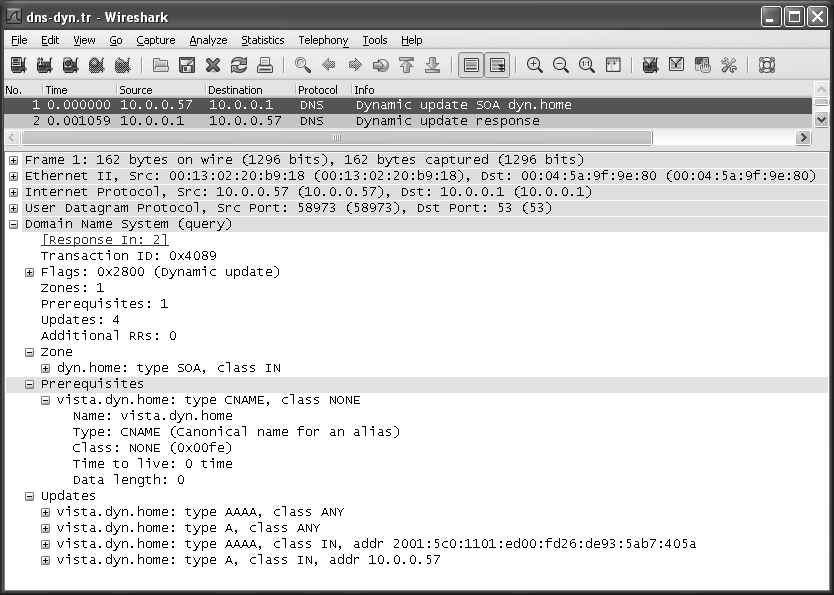
\includegraphics[width=0.7\textwidth]{imgs/11/11-16.png}
	\caption{DNS动态更新包含区域区段中的SOA记录和更新区段中的RR。这种情况包含主机 vista.
            dyn.home 的新的IPv4 和 IPv6地址}
\end{figure}

图11-16显示了动态更新是如何编码的。在10.0.0.1 的DNS服务器(本例中运行
BIND9[AL06])配置允许动态更新。区域区段包含识别要被更新的区域(vista.dyn.home)的
SOA记录。先决条件区段包含一个 RR,其RDATA 区段长度为0,TTL 值为0。RR 对应于
表11-5中第3行(RRset 不存在)的先决条件类型,因为它的类型不是ANY(为CNAME),
它的类被设置为 NONE(254)。

在这种特情况下,地址10.0.0.57和 2001:5c0:1101:ed00:fd26:de93:5ab7:405a 与名称
vista.dyn.home 相关联。通过首先删除AAAA 和A RRSet(对应于表11-6中第2行),然后将
AAAA 和A RRSet(对应于表11-6中第1行)添加到所需的地址,这样就可以完成。

DNS更新的响应很简单、紧凑。图11-16所示的更新的响应在图11-17中说明。

标志字段表示更新成功(没有错误)。事务ID(0x4089)用于确保更新的响应与对应的请
求相匹配。注意,在 Linux上,nsupdate 程序可以用来更新合作的DNS服务器。只有当授权
和访问控制过程说明请求是可以接受的,DNS服务器才与需求的更新协作。这可能简单如无
物,或在服务器上列出客户端的IP 地址,两者都不安全,或者可以使用更加复杂和安全的方
法,这些方法提供了事务认证 (transaction authentication)(见第18章中的 TSIG 和 SIG (0))。

\begin{figure}[!htb]
    \centering
	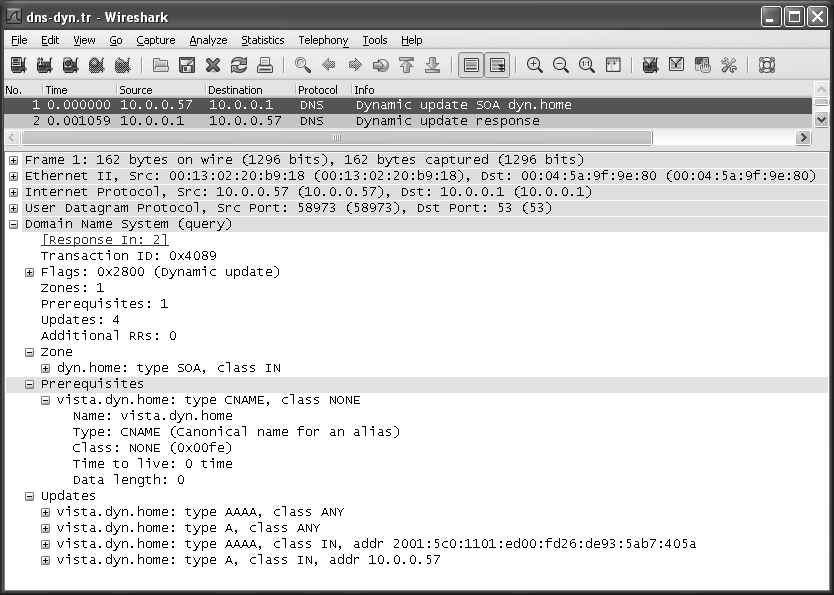
\includegraphics[width=0.7\textwidth]{imgs/11/11-16.png}
	\caption{对动态更新请求的响应包括一个事务ID 和状态标志集合}
\end{figure}

\subsection{区域传输和 DNS 通知}

区域传输用于从一个服务器到另一个服务器复制一个区域的一组RR(通常是从主服务
器向从服务器)。这样做的目的是保持多台服务器的区域内容同步。如果一台服务器失效了,
多台服务器可以为失败提供恢复能力。由于多台服务器能够共享传人查询的处理负载,性能
也可以改进。最后,如果服务器放置于离客户端近的地方,DNS查询/ 响应的延迟可能降低
(即解析器和服务器之间的网络延迟是很小的)。

按照最初的规定,区域传输在轮询(polling)后开启,在轮询中,从服务器周期性地联
系主服务器,通过比较区域的版本号以查看区域传输是否为必要的。稍后的方法认为,如果
需要开启区域传输,当区域内容改变时使用异步更新机制。这被称为 DNS NOTIFY。一旦启动
区域传输,或是传输整个区域(使用 DNS AXFR消息)\href{https://www.rfc-editor.org/rfc/rfc5936}{[RFC5936]},或是选择使用增量区域传输
(incremental zone transfer)(使用 DNS IXFR 的消息)\href{https://www.rfc-editor.org/rfc/rfc1995}{[RFC1995]}。一般方案根据图11-18所示进行
操作。

现在,我们将仔细查看每个选项,包括完整和增量区域传输,以及 DNS通知。

图11-18
DNS 区域传输在服务器之间复制
内容。一个可选的通知可以引起从
服务器请求完整或增量区域传输

\subsubsection{完整区域传输(AXFR消息)}

完整区域传输由区域的SOA 记录中的区域
传输参数控制:主名称服务器,序列号,刷新间
隔,重试间隔和到期间隔。当配置后,从服务器
尝试联系主服务器以查看区域传输是否是必要的。根据刷新间隔,周期性地尝试联系。当服
务器开启时,它们也开始尝试。如果联系没有成功(从服务器没有响应),根据重试间隔(一
般比刷新间隔短),周期性地尝试重试。如果在到期间隔内没有刷新,整个区域的内容被刷
新,同时使区域服务器无效。

一个全区域传送(AXFR)DNS信息(在问题区段包含AXFR类型的标准查询)使用
TCP 请求一个完整的区域传输。为了查看这样的消息,我们可以在本地网络中使用 host程序
来开始一个请求:

\begin{verbatim}
    Linux% host -1 home.
    Using domain server:
    Name: 10.0.0.1
    Address: 10.0.0.1#53
    Aliases:

    home name server gw.home.
    ap.home has address 10.0.0.6
    gw.home has address 10.0.0.1
    ...
\end{verbatim}

-l标志告诉host 程序从本地 DNS服务器执行一个完整区域传输。该程序启动一个基于 TCP
的查询/响应对话,如图11-19所示。


\begin{figure}[!htb]
    \centering
	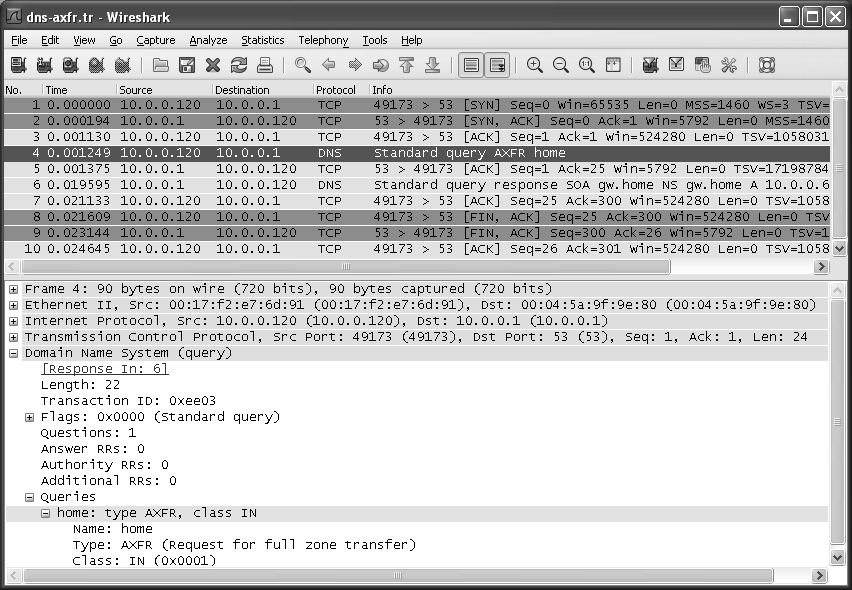
\includegraphics[width=0.7\textwidth]{imgs/11/11-19.png}
	\caption{一个完整区域传输的 DNS请求使用 AXFR 记录类型和 TCP 传输协议}
\end{figure}

在图11-19中,我们可以看到使用TCP的区域传输是如何发生的。前面的三个 TCP报
文段是标准TCP连接建立过程的一部分(见第13章)。第4个(解码)分组是请求。这是一
个正规的DNS标准,类型为AXFR,类为IN(互联网)。该查询是对于域名 home的。对于
该查询的响应包含在消息6中,跟随在TCP ACK 之后(见图11-20)。

在图11-20中,我们可以看到整个区域是如何在响应中运载的。在接收响应后,客户
端的TCP确认(ACK)数据,并且启动一个TCP连接关闭。使用FIN-ACK 握手(分组
8 ~10),连接被优雅地关闭了。查看第13章来获取关于标准TCP连接建立和清除的详细
情况。

\begin{figure}[!htb]
    \centering
	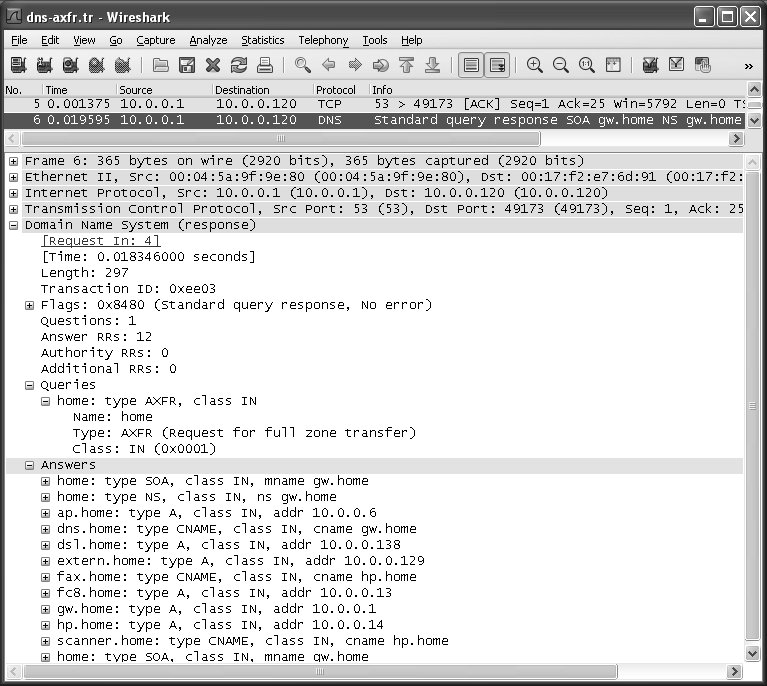
\includegraphics[width=0.7\textwidth]{imgs/11/11-20.png}
	\caption{完整区域传输请求的成功响应包括该区域的所有记录。事务使用TCP 进行,
            因为区域内容可能很大,并且需要一个可靠的副本}
\end{figure}

虽然它可以和任意的DNS服务器执行这样的区域传输,但是它们现在通常限制于区域
的权威服务器(例如,区域的NS记录中列出的那些)。该限制是出于隐私和安全的考虑一
区域内主机的知识可帮助对于特定服务或主机的攻击。

\subsubsection{增量区域传输(IXFR 消息)}

为了改进区域传输的效率,\href{https://www.rfc-editor.org/rfc/rfc1995}{[RFC1995]}定义了增量区域传输(incremental zone transfer)
的使用。使用增量区域传输和 IXFR消息类型,只提供区域中的变化。为了执行增量区域传
输,客户端(例如,从服务器)必须提供它在该区域的当前序列号。在下面的例子中,我们
可以通过提供序列号和dig 程序来模拟请求服务器:

\begin{verbatim}
    Linux% dig +short @10.0.0.1 -t ixfr=1997022700 home.
    gw.home hostmaster.gw.home. 1997022700 10800 15 604800 10800
\end{verbatim}

命令行中指出,命令的输出应该是简短的,10.0.0.1是要使用的DNS服务器的地址,以
序列号1997022700开始的增量区域传输应该被执行。这个例子创建了与图11-19 和图11-20
中所示的 AXFR类似的交换,只不过在这种情况下请求的序列号与当前的序列号匹配(见
Ele

\begin{figure}[!htb]
    \centering
	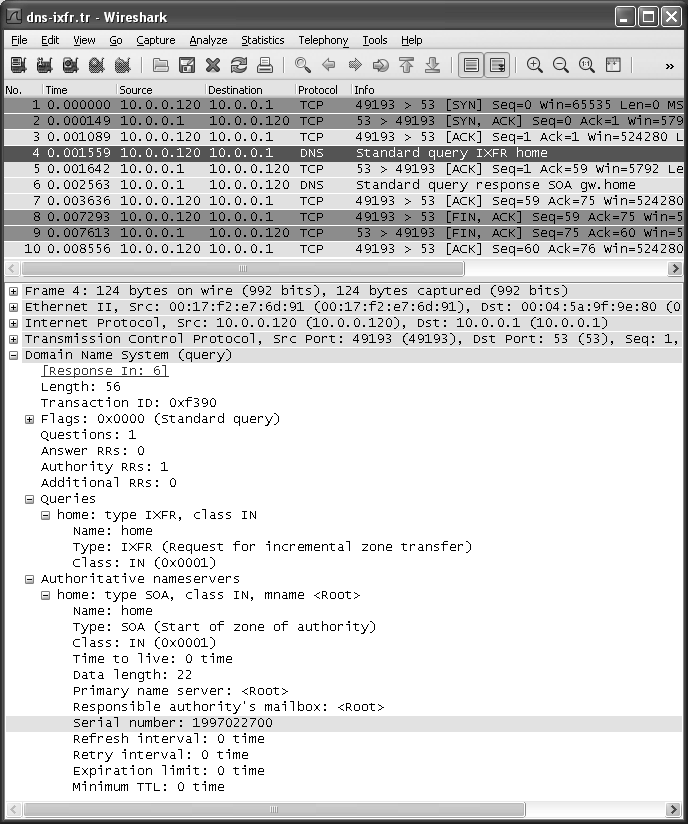
\includegraphics[width=0.7\textwidth]{imgs/11/11-21.png}
	\caption{在TCP 上运载的增量区域传输请求(IXFR记录类型)。序列号用于确定自前一次区域传输
            发生后哪些记录(如果有)已经改变了}
\end{figure}

图11-22显示了IXFR 请求如何在授权区段包含一个大多数空的SOA RR。SOA 记录
包括指定的序列号(1997022700)。响应(分组6)不包含任何真实的信息,因为序列号与
当前服务器的相匹配。

在图 11-22中的响应只在回答区段包含SOA RR。不像包含在查询中的那个,这个由完
整的SOA 字段填充(例如,邮箱、区域传输参数)。然而,没有额外的回答,因为当前该区
域的序列号与请求的序列号相匹配。因此,请求客户端被认为是最新的,而不需要任何额外
的信息或区域传输。

\subsubsection{DNS NOTIFY}

如前所述,轮询通常用于确定区域传输的必要性,也就是说,从服务器会定期(刷新间
隔)检查主服务器,查看区域是否已经更新(通过不同的序列号说明),在哪种情况下区域传
输将启动。这个过程有点浪费,因为许多无用的轮询在区域更新前可能发生。为了改善这种
情况,\href{https://www.rfc-editor.org/rfc/rfc1996}{[RFC1996]}DNS设计了 DNS NOTIFY 机制。DNS NOTIFY 允许修改区域内容的服务
器通知从服务器更新已经发生,区域传输应该启动。更具体地说,如果启用,当区域SOA
RR 改变(例如,如果序列号增加)时,通知消息被发送到一组感兴趣的服务器。这使得区域
传输在需要时开启。使用本地名称服务器,我们可以看到这是如何工作的(见图11-23)。

\begin{figure}[!htb]
    \centering
	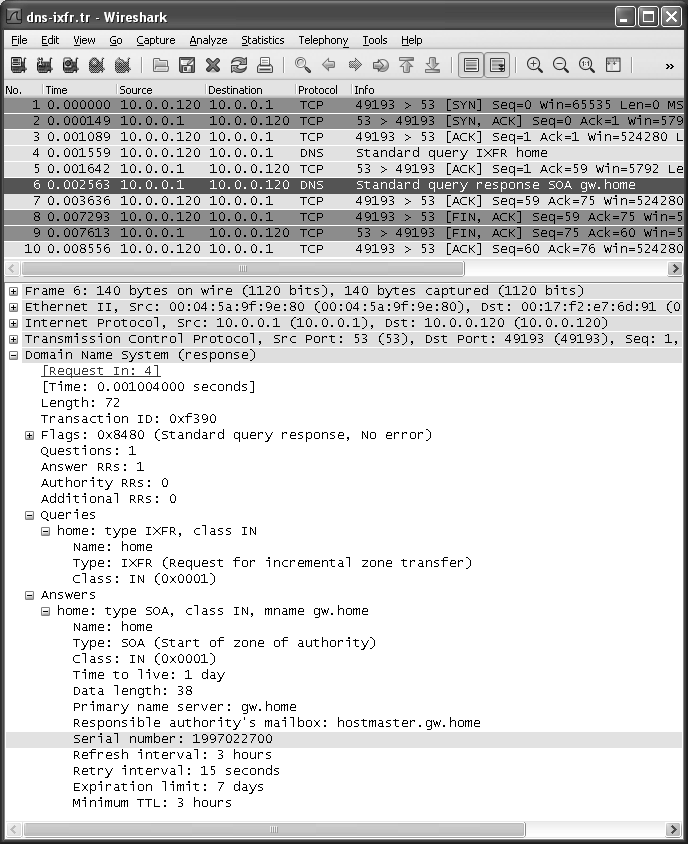
\includegraphics[width=0.7\textwidth]{imgs/11/11-22.png}
	\caption{当序列号是当前的时,IXFR请求的响应只包含一个 SOA记录,没有额外的信息}
\end{figure}

这个例子说明了简单的 DNS NOTIFY 消息,它被发送到服务器的通知服务器集合之
中的一台主机,该通知服务器集合由应该被通知区域改变的服务器组成。消息是一个UDP/
IPv4 的DNS 查询消息,其标志字段说明区域变化通知。查询区段包含一个 SOA记录的类型
和类,回答区段包含该区域的当前 SOA RR(TTL *0),包括序列号。这为通知服务器提供
足够的信息,以确定区域传输可能是必要的。需要注意的是,一个服务器可能从多个其他服
务器收到通知,此时它们在更新其区域信息。这对于协议操作不存在问题。

DNS NOTIFY 机制默认使用UDP,UDP 是一种不可靠的协议。在特殊的例子中,通知
集合只包括地址10.0.0.11,它不运行 DNS服务器。因此,消息每隔15s重发一次,以希望
获得从来不会到达的响应。

\begin{tcolorbox}
    重发之间的时间以及尝试重发的总数,在\href{https://www.rfc-editor.org/rfc/rfc1996}{[RFC1996]}中分别建议为60s和
    5次。它还建议使用一种计时补偿方法(递增或指数级)。在这里我们可以看到的
    BIND9 并没遵循这些建议,因为两次重传间隔15s。
\end{tcolorbox}

\begin{figure}[!htb]
    \centering
	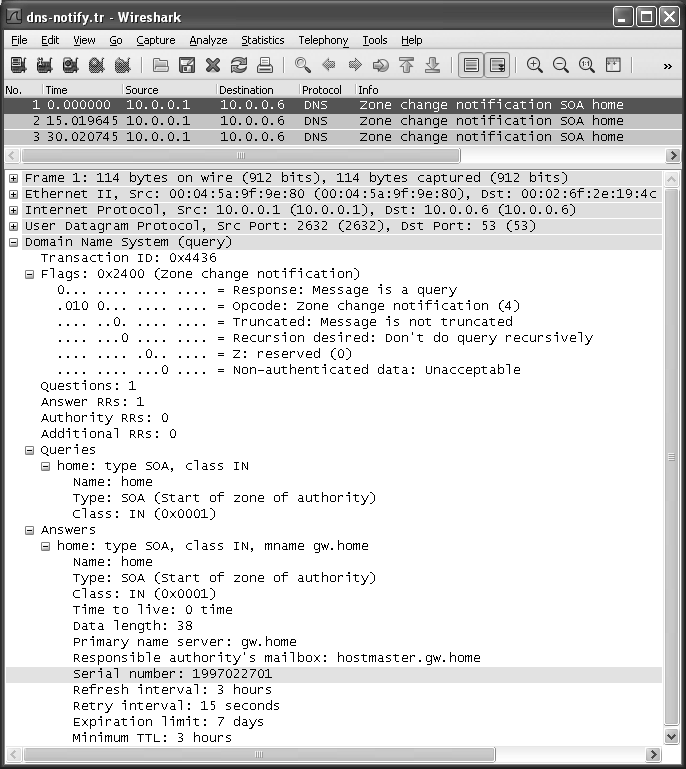
\includegraphics[width=0.7\textwidth]{imgs/11/11-23.png}
	\caption{一个 DNS NOTIFY,说明区域文件的更新。间隔 15s有两个重传(与标准中建议的方法相反)}
\end{figure}

响应是简单的DNS响应消息,除了事务ID外没有有用的信息;它们只用于完成协议以
及取消发送服务器的重传。

\section{排序列表、循环和分离 DNS}

到目前为止,我们已经讨论了如何设置域名,DNS支持的资源记录类型,以及用于获取
和更新区域的DNS协议。需要考虑的一点是,返回什么样的数据以及以什么样的顺序响应
DNS查询。DNS服务器可以返回所有匹配的数据给任何客户端,并以服务器认为最方便的
顺序返回。然而,特殊的配置选项和行为在大多数 DNS服务器软件中是可用的,以达到一
定的操作、隐私或性能目标。考虑图11-24所示的拓扑结构。

图11-24所示的拓扑结构类型是典型的小型企业的。有一个私有网络和一个包括 DNS
服务器的公共网络。此外,在DMZ上有一对主机(A和B),在内部网络上有一个(C),在
互联网上有一个(R)。多宿主主机(M)跨越 DMZ 和内部网络。因此,M 有来源于两个不
同网络前缀的 IP 地址。

一台希望联系 M 的主机执行 DNS查找,返回两个地址,一个与内部网络相关,一个与
DMZ相关。当然,如果A、B和R通过DMZ到达M,C通过内部网络到达M,这将更高效。
一种普遍会发生的情况是,DNS 服务器基于请求的源IP 地址排序它返回的地址。(也可以使
用目的IP 地址,尤其是如果M在相同的网络接口上使用来自不同子网的多个IP 地址。)如
果请求系统使用和返回地址记录的源具有相同的网络前缀的源IP 地址,DNS服务器在返回
的消息中早一些放置这样的匹配记录的集合。这种行为鼓励客户端找到它正尝试联系的特定
的服务器的“最近的”IP地址,因为大部分简单的应用程序尝试联系返回地址记录中发现的
第一个地址。这种精确的行为可以通过使用所谓的 sortlist 或是 rrset-order 指令来控制(解析
器和服务器的配置文件中使用的选项)。如果由 DNS 服务器软件默认执行,这样的排序行为
也可能自动发生。

图11-24 在小型企业的拓扑结构中,DNS 可以配置返回为依赖于请求IP 地址的不同的地址

当多台服务器提供一种服务时,传人的连接就会是负载均衡的(即,在服务器之间划
分),这时一些相关的问题就会出现。在前面的例子中,想象一个服务由A和B提供。这样
的服务可以通过URL http://www.example.com来识别。请求客户端(如R)执行域名 www.
example.com 的DNS查询,并且 DNS服务器最终返回一个地址记录的集合。要实现负载均
衡,DNS服务器可以配置为使用DNS循环(round-robin),这意味着服务器交换返回地址记
录的顺序。这样做鼓励每个新的客户端访问不同于前一个客户端服务器上的服务。虽然这有
助于平衡负载,但是这远不够完美。当记录被缓存时,预期的效果可能因复用现有的缓存
地址记录而不会发生。此外,这种方案可以很好地平衡跨服务器连接的数量,但不是负载。
不同的连接可以有完全不同的处理要求,因此真正的处理负荷可能始终保持不平衡,除非特
定的服务总是具有相同的处理要求。

最后的考虑是关于DNS服务器返回的数据支持隐私的问题。在这个例子中,我们希望
安排该企业内的主机能够检索网络中的每一台计算机的资源记录,同时,我们限制对R可见
的系统的集合。为实现这一目标,有一种称为分离 DNS(split DNS)的技术。在分离 DNS
中,响应查询的返回的资源记录集合依赖于客户端的身份,并可能查询目的地址。大多数
情况下,客户端由IP地址或地址前缀确定。使用分离 DNS,我们可以安排企业的任何主机
(即那些共享一组前缀的)配备整个 DNS数据库,而那些外面的只能看见A和B,其中提供
了主要的Web服务。

\section{开放 DNS 服务器和 DynDNS}

许多家庭用户由他们的ISP分配一个单一的IPv4地址,这个地址随用户的电脑或家庭
网关连接、断开和重新连接到互联网而改变。因此,用户往往难以建立一个 DNS条目,允
许运行的服务对互联网是可见的。一些所谓的开放动态 DNS(Dynamic DNS,DDNS)服务
器可以用来支持特殊的更新协议,称为DNS 更新 API [DynDNS],凭此,用户可以根据预
先注册或账户在提供商的 DNS服务器中更新条目。这项计划不使用前面所述的「RFC21361
DNS UPDATE 协议,反而是一个独立的应用层协议。

为了使用这项服务,在客户端系统上运行 DDNS客户端程序(例如,Linux 中的 inadyn
或 ddclient 以及 Windows 的 DynDNS Updater),也可能是在用户的家用路由器上。大多数情
况下,这些程序被配置为需要登录信息,以用于访问远程DDNS服务。当服务被调用时,客
户端程序与服务器联系,提供它的主机的当前全球IP 地址(由ISP 分配的一个,往往是一个
NAT映射的地址),并且变静态。之后,它会定期更新与服务器的信息。这样做允许服务
器在某个时间间隔内没有接收到更新时清除信息。这些服务包括在以下 Web 网站中提供的
服务(截止到2011年):http://www.dyndns.com/services/dns/dyndns, http://freedns.afraid.org
和 http://www.no-ip.com/services/managed\_dns/free\_dynamic\_dns.html。

\section{透明度和扩展性}

DNS 是互联网上最普遍的服务之一,并已成为一个有吸引力的服务,它通常作为基础,
通过扩展添加新的功能。例如,有很多记录类型,如TXT.SRV 和A(例如,见\href{https://www.rfc-editor.org/rfc/rfc5782}{[RFC5782]}),
可以用来为未来的服务编码有用数据。\href{https://www.rfc-editor.org/rfc/rfc5507}{[RFC5507]}为扩展 DNS设想了各种方法,最终结论
是建立和实现新的 RR类型是最有吸引力的办法。多亏了较早的规范\href{https://www.rfc-editor.org/rfc/rfc3597}{[RFC3597]},有一种标
准方法将未知的 RR类型作为不透明的数据来处理。也就是说,如果不认可,它们不解释,
处理是透明(transparent)的。这允许新的 RR类型在运载时不会对现有 RR类型的处理造成
负面影响。

保持透明度存在的问题之一是嵌人域名的编码和压缩。对于已知的RR类型,为了使用
压缩标签实现压缩,允许改变嵌入域名的大小写。拥有者域名(查询的“关键字”)总是服从
于压缩。然而,对于未知的RR类型,嵌人的域名不得使用压缩标签。此外,将来包含嵌人
域名的RR类型也同样禁止(见\href{https://www.rfc-editor.org/rfc/rfc3597}{[RFC3597]}的第4节)。未知类型仍然可以按位进行比较(例
如,动态更新)。这意味着,任何嵌人域名以大小写敏感的方式相比较\href{https://www.rfc-editor.org/rfc/rfc4343}{[RFC4343]},这与大
多数其他的DNS操作相反。同样的情况也出现在使用TXT记录的嵌入域名中。

当新形势的服务和处理DNS流量的代理引入时,另一个与透明度相关的问题出现了。
如今在一个家庭网关或防火墙内部包含一个 DNS代理是相当普遍的。一个典型的代理处理
来自于用户家庭网络的传人DNS请求,并将该请求转发到ISP 提供的域名服务器。它也接
收返回的信息,并可以(也可以不)缓存结果。从历史上看,一些代理试图做的不仅仅是中
继请求和答复,这已经引起了一些与 DNS的互操作性的问题。\href{https://www.rfc-editor.org/rfc/rfc5625}{[RFC5625]}指定了 DNS代理
的合理的操作,基本上要求 DNSRR 是无解释的,并仅仅由代理中继。数据分组被截断的情
况是无法避免的,任何这样的代理必须设置TC位字段表明一些 DNS数据被删除了。此外,
任何此类代理应准备处理TCP 请求,因为当基于 UDP 的请求被截断时,这是传统的回退机
制,并且由\href{https://www.rfc-editor.org/rfc/rfc5966}{[RFC5966]}要求。

\section{从IPV4 向 IPV6 转换 DNS}

第7章中我们描述了一个框架,用于在IPv4 和IPv6 之间转换 IP 数据报。支持这种能
力的转换器预计将与在 DNSA 和 AAAA 记录之间转换的相关功能一起部署\href{https://www.rfc-editor.org/rfc/rfc6147}{[RFC6147]},后
者允许只有IPv6 的客户端来访问出现在A记录中的DNS信息(例如,在IPv4 互联网中)。
这种功能被称为 DNS64,其建议的部署方案之一(称“DNS递归解析模式中的 DNS64”
如图 11-25所示

图 11-25 DNS64将A记录转换为 AAAA 记录,并和 IPv4/IPv6 转换器一起工作,
以允许只有 IPv6 的客户端访问 IPv4 网络中的服务

如图 11-25所示,DNS64 和 IPv4/IPv6转换器结合使用(见第7章)。每个设备配置一
个或多个通用IPv6 前缀,这些前缀是在创建嵌人式IPv4地址中使用的。每个前缀可能是
一个网络特定的前缀(例如由运营商拥有)或是知名前缀(64:ff9b::/96)。DNS64设备作
为一个缓存DNS服务器。只有IPv6 客户端使用它作主 DNS服务器,并可以请求域名的
AAAA 记录。DNS64将这样的请求转换为IPv4端的A 和 AAAA记录的请求。如果没有返
回AAAA 记录,基于配置的前缀和它检索的每个A记录的内容,DNS64通过形成嵌人式
IPv4 地址来提供合成(synthetic)AAAA 记录。DNS64 也响应它用于合成AAAA RR 的任意
IPv6地址的PTR 查询。

为了在DNS64设备中实现 AAAA RR 的合成,只实际改变 DNS消息的回答区段。其他
区段仍然与在IPv4端检索时一样。当是 CNAME 或DNAME 链时,链递归地跟随,直到发
现A 或AAAA 记录为止,并且链的元素会在响应中包含。此外,可以配置 DNS64,以便避
免特的排除IPv6或IPv4地址范围的合成。这防止了某些异常行为(例如,基于特殊用途
的IPv4地址形成嵌人式IPv4地址)。请注意,DNS64与DNSSEC 有微妙的相互作用,这些
问题在第18章中涉及。

\section{LLMNR 和 MDNS}

普通的DNS 系统需要配置一组 DNS服务器以提供名称和地址之间的映射,以及其他可
能的信息。当只有少数本地主机希望通信时,有时这开销太大。在DNS服务器不可用的情况
下(例如,迅速形成的客户端的 ad hoc(自组织)网络,只是相互连接),可以使用一个特殊的
DNS 本地版本,称本地链路组播名称解析(Link-Local Multicast Name Resolution, LLMNR)
\href{https://www.rfc-editor.org/rfc/rfc4795}{[RFC4795]}。它是一个由微软开发的基于DNS的(非标准)协议,并在本地环境中使用以帮
助发现局域网上的设备,如打印机和文件服务器。Windows Vista、 Windows Server 2008 和
Windows 7中都支持它。对于IPv4 组播地址224.0.0.252 和 IPv6地址 ff02::1:3,它使用UDP
端口 5355。如果来自它们响应的任何单播IP 地址,服务器也可以使用 TCP 端口 5355。

组播 DNS(multicast DNS,mDNS) [IDMDNS]是另一种形式的本地类 DNS 功能,它
是由苹果公司开发的。当它和 DNS 服务发现协议结合时,苹果称之为框架 Bonjour。mDNS
使用通过本地组播地址携带的DNS消息,使用 UDP 端口 5353,规定特殊的TLD.local 用特
殊的语义处理。.local TLD 在本地链路范围。在该TLD 中的域名的任何 DNS查询被发送到
mDNS IPv4地址224.0.0.251或IPv6地址 f02::1b。对于其他域的查询可以随意发送到这些
组播地址。允许本地链路服务器来响应全局名称的映射可能引起重大安全问题。为了解决这
一问题,可以使用 DNSSEC(见第18章)。mDNS 支持在.local 伪TLD 中自主分配名称,尽
管这种伪TLD 还没有被正式预留\href{https://www.rfc-editor.org/rfc/rfc2606}{[RFC2606]}。因此,诸如家庭局域网等小型网络上的主机
可以被分配合适的名称,如 printer.local、fileserver.local、cameral.local、kevinlaptop.local 等。
mDNS 中的机制用于检测和解决冲突。

\section{LDAP}

到目前为止,我们已经讨论了 DNS和类似于DNS的本地名称服务。为了支持更丰
富的查询和数据操作,有一种更普遍的目录服务,即我们前面提到的称为LDAP的服务
\href{https://www.rfc-editor.org/rfc/rfc4510}{[RFC4510]}。LDAP(现在 LDAPv3)是一种互联网应用层协议,可以根据 X.500(1993)[X500]
数据和服务模型提供对于一般目录的访问(例如,“白页”)。它提供了搜索、修改、添加、比
较和删除基于用户选择模式的条目的能力。LDAP 目录是一个目录条目的树,每个条目包含
一组属性。由于 TCP/IP 已更受欢迎,LDAP已经从根源演进为与DNS一起工作。例如,与
MIT 的校长办公室匹配的目录查询可以通过使用 LDAP搜索工具 Idapsearch(微软有一个与之
相当的工具称为ldp,在它的web 站点作支持工具提供)来形成,它按如下方式工作:

\begin{verbatim}
    Linux% ldapsearch -x -h 1dap.mit.edu -b "dc=mit,dc=edu" \
    "(ou=*Chancel1or*)"
    # extended LDIF
    #
    # LDAPV3
    # base <dc=mit,dc=edu> with scope sub
    # filter: (ou=*Chancellor*)
    # requesting: ALL
\end{verbatim}

命令行说明服务器Idap.mit.edu 可以不使用任何特殊的验证协议来联系(-x选项)。虽
然LDAP 的完整讨论远远超出了本章(和本书)的范围,但部分输出显示了dc(域组件)属
性如何被用来链接LDAP数据和 DNS。每个dc 组件拥有一个 DNS标签,并且它们可以被
用来编码一个完整的域名,这被用作LDAP 查询的“基础” 部分。使用本约定,形成有效的
LDAP 查询并不特别困难。在这种情况下,它是包含单词 Chancellor 的组织单位(ou)。请注
意,可以使用通配符。

LDAP 服务器经常在企业内部用于保留目录信息,如位置、电话号码和组织单位。微软
的活动目录产品包含LDAP 的功能,被广泛用于管理用户账户、服务,以及使用 Windows
的大企业中的访问权限。一些LDAP服务器(如 MIT 的和其他许多大学的)也可通过公共互
联网使用。

\section{与DNS相关的攻击}

DNS是互联网的一个重要组成部分,多年以来它已经成为一些攻击和对策的对象
\href{https://www.rfc-editor.org/rfc/rfc3833}{[RFC3833]}。最近,在添加强认证到 DNS操作中方面,DNS 安全(DNSSEC)这项全球性工
作已取得实质性进展。我们将 DNSSEC如何工作的详细讨论推迟到第18 章,其中我们也涉
及必要的密码学背景。现在,我们探索对 DNS已经发动的一些攻击。

对DNS的攻击有两种主要的形式。第一种形式涉及 DoS攻击,在这类攻击中,由于重
要DNS 服务器(如根或 TLD服务器)过载,DNS 不起作用。第二种形式改变资源记录的内
容,或伪装成一个官方 DNS 服务器,但是回复假的资源记录,从而导致主机在尝试与另一
台机器连接时,连接至错误的IP 地址(例如,银行的Web 站点)。

2001年年初发生了第一次针对DNS的重大DoS攻击。攻击包含生成很多对 AOL.
COM的MX记录的请求。攻击者使用伪造的源IP 地址产生对于MX记录的DNS请求。请
求是一个相对较小的数据分组,然而响应较大(约20倍),因此这种类型的攻击被称为放大
(amplifcation)攻击—因为攻击造成的结果是,消耗的带宽量比生成攻击所占的带宽量要
大很多。响应会定向到请求分组中包含的IP地址,所以攻击者基本上可以导致响应流量定
向到任何他想要的地方。攻击在CERT事件记录中详细陈述[CIN]。

一种形式的攻击涉及 DNS中数据的修改,这在2008年年底有报道[CKB],现在被称为
Kaminsky 攻击。它包含缓存中毒(cache poisoning),在这种攻击中,一台DNS服务器的缓
存内容被错误的或伪造的数据替代,并且最终送达终端主机上的解析器。它的一个变种是,
攻击者使用特定主机域名的域的 NS记录来响应一台缓存服务器的A记录的查询。主机的IP
地址(由攻击者所选择的)也在DNS 响应的额外信息区段中提供。主机域名可能共享也可能
不共享相同的子域作为原始的 DNS请求。与这种形式的攻击相关的主要风险是,依赖于合
适的 DNS名称到地址解析的客户端可能被定向到伪服务器。如果这样的服务器被故意配置
为模仿原来的主机(例如,伪装成银行的Web 服务器),用户可能会无意地信任伪装的服务
器,并泄露敏感信息。对此以及其他相关攻击的缓解技术在\href{https://www.rfc-editor.org/rfc/rfc5452}{[RFC5452]}中给出。一种方法没
有在\href{https://www.rfc-editor.org/rfc/rfc5452}{[RFC5452]}中描述,称为 DNS-0x20[D08],它涉及编码问题区段查询名称部分每个字
符的0x20位置的临时值,该问题区段会在每个响应的对应位置中回显。这成为可能,因为,
虽然域名以大小写不敏感的形式比较,当形成响应时,服务器往往会返回一个查询名称的完
全相同的副本。如果在查询中拥有者的名称大小写故意混排,主动响应将难以重新产生临时
值,并且更容易被识别(和忽略)。

\section{总结}

DNS 是互联网的一个重要组成部分,DNS技术也被广泛应用于私有网络中。DNS名称
空间是全世界范围的,并且划分成以顶级域名开始的层次结构。域名可以使用国际化域名
(IDN)以多种语言和文字表示。应用程序使用解析器来联系一个或多个 DNS服务器,执行
对区域数据库的查找任务,如转换主机名称到一个 IP 地址,反之亦然。解析器然后联系一
个本地域名服务器,该服务器可能递归地联系一个根服务器或满足该请求的其他服务器。大
多数 DNS 服务器和一些解析器缓存知道的信息,在一段称为生存时间(TTL)的间隔内,将
其提供给随后的客户端。查询和响应使用一个特殊的DNS协议,它与TCP或UDP一起工
作。协议也可以与IPv4或IPv6 协议或两者的混合物一起工作。

所有的 DNS查询和响应有相同的消息格式,包括问题、回答、授权信息和额外信息。
资源记录用来保存大部分的DNS信息,这样的类型有许多:地址,邮件交换站,名称的
指针等。在互联网上,大多数DNS消息使用UDP/IPv4传输,并且被限制为512个字节的
长度,但是一种特的扩展选项(EDNSO)提供了更长的消息,要求支持DNS安全协议
(DNSSEC),我们将在第18章中详细讨论。

DNS 支持一些特殊的功能,如区域传输和动态更新。区域传输(完整或增量)用于允许
冗余的从服务器与主服务器同步区域的内容,主要是为了冗余。动态更新允许应用程序使用
在线协议修改区域的内容。事实上这种功能有两种形式:一种由\href{https://www.rfc-editor.org/rfc/rfc2136}{[RFC2136]}标准化,并在企
业使用;一种是非标准的但非常流行的动态 DNS功能,它允许用户分配临时 IP地址(例如电
缆或DSL)来获得一个 DNS 条目,所以它们提供的服务可以通过遍及全世界
DNS一直受到众多攻击,从DoS 攻击(它使得DNS仅有有限的能力
毒攻击(它可使恶意的服务器显得如合法的)。已经提出各种技术来解决这
密技术(第18章涵盖)和修改DNS服务器以减少接收未经请求的 DNS 响应

\section{参考文献}

[AL06] P. Albitz and C. Liu, DNS and BIND, Fifth Edition (O'Reilly Media, Inc,
2006).

[CIN] http://www.cert.org/incident\_notes/IN-2000-04.html

[CKB] http://www.kb.cert.org/vuls/id/800113

[D08] D. Dagon et al., "Increased DNS Forgery Resistance Through Ox20-bit
Encoding" Proc. ACM CCS, Oct. 2008.

[DNSPARAM!http://www.iana.org/assignments/dns-parameters

[DR97] D. Dougherty and A. Robbins, sed \& awk, Second Edition (O'Reilly Media,
1997).

[DYNDNS] http://www.dyndns.com/about/technology

[ENUM] http://www.iana.org/assignments/enum-services

IGTLD] http://www.iana.org/domains/root/db

IICANN] http://www.icann.org/en/tlds

[IDDN] S. Rose and W. Wijngaards, "Update to DNAME Redirection in the
DNS," Internet draft-ietf-dnsext-rfc2672bis-dname, work in progress, July 2011.

[LDIMDNS] S. Cheshire and M. Krochmal, "Multicast DNS," Internet draft-
cheshire-dnsext-multicastdns, work in progress, Feb.2011.

[IDN] http://www.icann.org/en/topics/idn

[ISO3166] International Organization for Standardization, "International Stan-
dard for Country Codes,” ISO 3166-1, 2006.

[ISPR] http://www.iana.org/assignments/service-names-port-numbers

[021 J. Jung et al.,"DNS Performance and the Effectiveness of Caching" IEEE/
ACM Transactions on Networking, 10(5), Oct. 2002.

[MD88] P. Mockapetris and K. Dunlap, "Development of the Domain Name Sys.
tem/” Proc.ACM SIGCOMM, Aug. 1988.

[P10] N. Paskin, "Digital Object Identifier (DOIO) System,' Encyclopedia of Librar
and Information Sciences, Third Edition (Taylor and Francis, 2010).

[R06] H. Rice, "ENUM—The Mapping of Telephone Numbers to the Internet"
The Telecommunications Review, 17, Aug. 2006.

[ROOTS] http://www.root-servers.org

[RSYNC] http://rsync.samba.org

[SNPJ http://www.iana.org/assignments/s-naptr-parameters

[U11] The Unicode Consortium, The Unicode Standard, Version 6.0.0 (The Unicode
Consortium,2011).

[URI] http://www.iana.org/assignments/uri-schemes

[URN] http://www.iana.org/assignments/urn-namespaces

[X500] International Telecommunication Union—Telecommunication Standard-
ization Sector, "The Directory—Overview of Concepts, Models and Services,"
11U-T X.500, 1993